\chapter[Neutral carbon in high-redshift radio galaxy gas haloes]{Molecular hydrogen kinematics and masses traced by neutral carbon in $z \gtrsim 2.9$ radio galaxies}\label{chapter4}
% Edit THIS version

% Abstract of the paper
\section*{Abstract}
We have used atomic carbon, [\ion{C}{i}]($^3$P$_1 - ^3$P$_0$), or more simply, [\ion{C}{i}](1-0), to trace molecular hydrogen (H$_2$) within seven high redshift radio galaxies (HzRGs) and their extended gas haloes. [\ion{C}{i}](1-0) line emission is frequently used to trace H$_2$ in low gas density and metallicity regions where cosmic ray energy densities are high enough to cause wide-scale photodissociation of $^{12}${CO} which also traces H$_2.$ To probe H$_2$ within the diffuse circumgalactic region therefore, we obtain [\ion{C}{i}](1-0) line and continuum observations of the HzRG sample at redshifts of $2.9 \leq z \leq 4.6$ obtained using the Atacama Large Millimetre-submillimeter Array (ALMA). Although six out of the seven HzRGs do not have clear [\ion{C}{i}](1-0) detections at their nuclear regions, we are still capable of estimating $3\sigma$ upper limits for their H$_2$ masses. Assuming a nominal line width of $\rm FWHM = 100$ km s$^{-1},$ we obtain host galaxy H$_2$ masses in the order of $\rm M_{H_2} \lesssim10^{10}$ M$_\odot.$ The only detected [\ion{C}{i}](1-0) line emission at a host galaxy is for TN J0121+1320 at $z=3.52$ which has a line-width $\rm FWHM = 157 \pm 40$ km s$^{-1}.$ Furthermore, a blind search for [\ion{C}{i}](1-0) in the fields surrounding the host galaxies results in several detections being made. From them, we obtain H$_2$ masses in the order of $\rm M_{H_2} \simeq 10^9$ M$_\odot.$ The H$_2$ gas is traced at distances of $d \simeq 10 - 200$ kpc from the host galaxies and is thus part of the circumgalactic medium. The line-widths of the circumgalactic medium H$_2$ gas are within the range of $\rm FWHM \simeq 20 - 100$ km s$^{-1},$ implying kinematically quiet gas that is less turbulent than the gas traced in the interstellar medium of the host galaxy of TN J0121+1320. 

%%%%%%%%%%%%%%%%%%%%%%%%%%%%%%%%%%%%%%%%%%%%%%%%%%

%%%%%%%%%%%%%%%%% BODY OF PAPER %%%%%%%%%%%%%%%%%%

\section{Introduction}

%All papers should start with an Introduction section, which sets the work
%in context, cites relevant earlier studies in the field by \citet{Others2013},
%and describes the problem the authors aim to solve \citep[e.g.][]{Author2012}.

It is widely accepted that molecular hydrogen (H$_2$) is critical for star-formation in galaxies. Given the prevalence of carbon monoxide ($^{12}$CO or simply CO) within the giant molecular clouds from which stars form and the difficulty associated with detecting H$_2$ directly, CO lines have long been the primary tracers for H$_2$ within galaxies \citep{SolomonvandenBout2005}.

In addition to using CO to trace H$_2,$ efforts have been made to make use of other line tracers to trace H$_2$ gas clouds within and around galaxies. One of these is [\ion{C}{i}]$^3$P$_1 - ^3$P$_0,$ in short [\ion{C}{i}](1-0), which can be a better alternative for tracing H$_2$ within environments where CO molecules are photodissociated by cosmic rays and far-ultraviolet (FUV) radiation produced by star-formation \citep{Bisbas2015,Bisbas2017}. 

Observationally, motivation to use [\ion{C}{i}](1-0) as a H$_2$ tracer has been put forward by a pilot study of ultra-luminous infrared galaxies (ULIRGs) which found good agreement between H$_2$ masses inferred from [CI] and CO \citep{PapadopoulosGreve2004}. Despite giant molecular clouds being irradiated by cosmic ray energy densities ($\rm U_{CR}$) greater than those measured within star-forming regions in the Milky Way, i.e. $\rm U_{CR} \simeq (50 - 1000)~U_{CR,Gal}$, carbon atoms are unaffected by cosmic rays. The strength of [\ion{C}{i}] fine structure line emission is therefore preserved in gas regions of high cosmic ray energy density.

Further results presented in \citet{Papadopoulos2018} have confirmed that cosmic ray energy densities result in [\ion{C}{i}]-rich and CO-poor gas environments when star-formation rates and active galactic nuclei (AGN) activity are high, as well as in the vicinity of synchrotron radiation produced by radio jets. 

In light of this, several studies to date have made use of the [\ion{C}{i}] fine-structure lines, [\ion{C}{i}]$^3$P$_2$ - $^3$P$_1$ and [\ion{C}{i}]$^3$P$_1$- $^3$P$_0,$ [\ion{C}{i}](2-1) and [\ion{C}{i}](1-0), to trace H$_2$ gas. One such example is the first [\ion{C}{i}] survey of high-redshift ($z > 2$) sub-mm galaxies and quasar hosts of \citet{Walter2011}. There are a multitude of other examples of H$_2$ gas masses and dynamics being estimated for lensed star-forming/starburst high-$z$ galaxies \citep{Bothwell2017,Andreani2018,Lelli2018,Nesvadba2019}, a compact star-forming $z \simeq 2$ galaxy \citep{Popping2017} and sub-mm galaxies \citep{Alaghband-Zadeh2013}. 

[\ion{C}{i}] detections have been important tracers of H$_2$ in high-redshift radio galaxies (HzRGs) such as PKS 0529-549 at $z=2.57$ \citep{Man2019}. Within the extended halo of the Spiderweb Galaxy (MRC 1138-262 at $z\simeq2.16$), a giant HzRG engulfed by satellite galaxies, \citet{Gullberg2016b} detected line-broadened [\ion{C}{i}](2-1) emission at the galaxy's radio core as well as $d \simeq 4$ kpc from it. Prominent [\ion{C}{i}](1-0) emission has also been detected in the CGM of Spiderweb Galaxy at distances between $d \simeq 17$ and 70 kpc from its nucleus \citep{emonts2018}. 

One of the main advantages of [\ion{C}{i}] fine-structure lines are that they are optically thin hence their line surface brightness correlates well with the mass of neutral carbon within a given molecular cloud \citep{Nesvadba2019}. [\ion{C}{i}] lines also have a low enough critical density of $n_{\rm crit} = 500$ cm$^{-3}$ and are therefore able to trace diffuse, low density gas on the outskirts of galaxy haloes. The outlying halo gas is now commonly referred to as the circumgalactic medium (CGM) which has recently come into interest as a new frontier within which to study baryon flows into and out of galaxies. These studies have been encouraged by the development of high-sensitivity integral field unit (IFU) instruments with which it is now possible to detect diffuse and faint gas that extends out to hundreds of kpc from a galaxy nuclei \citep{tumlinson2017}. 

The ionised and molecular gas in the CGMs of HzRGs have also observed in extensive detail. Generally, the ionised component of the CGM is traced by rest-UV lines such as Ly$\alpha$ $\lambda1216$, \ion{C}{IV} $\lambda1550$, \ion{N}{V} $\lambda1240$ and \ion{O}{III]} $\lambda1660$ which both long-slit spectroscopy and IFU observations have shown to be vast, extending out to $d\sim200$ kpc in some galaxies \citep{reuland2003,villar-martin2003,humphrey2007,swinbank2015,morais2017,silva2018b}. 

Molecular gas within a number of HzRGs has already been traced using CO \citep{Emonts2011,Emonts2014,Gullberg2016b}. However, a CO survey for HzRGs has yet to be carried. Therefore, in the absence of a wide CO catalogue HzRGs, we carry out a pilot study of [\ion{C}{i}](1-0) in order to constrain the kinematics and masses of H$_2$ in the galaxies' ISM and CGM gas and gain a more complete view of both the ionised and molecular phases of the CGMs. The ALMA observations have targeted the [\ion{C}{i}](1-0) line. These milimetre/sub-milimetre observations are complemented by those of the VLT/MUSE (Very Large Telescope/Multi-unit Spectroscopic Explorer) IFU spectrograph which has a spectral range of $4650~\ang < \lambda < 9300~\ang$ and can detect rest-UV lines that trace the warm, ionised gas medium within haloes. The sensitivity, resolution and frequency coverage of ALMA make it a superb instrument for detecting H$_2$ tracers such as the [\ion{C}{i}](1-0).

In Section 2, we provide an overview of the data acquired and how it has been reduced. Section 3 explains the method for analysis. Section 4 describes the results. In Section 5, we explore the implications of our findings within the broader field of high-redshift galaxy evolution. Finally, in section 6, we summarise the main points of this study. We have used \citet{Planck2016} $\Lambda$CDM cosmology, throughout, under the following cosmological constraints $\rm H_0 = 67.8~km~s^{-1}~Mpc^{-1}$ and $\rm \Omega_m = 0.308.$ 

% - - - - - - - -
\section{Observations and Data Reduction}
\subsection{ALMA}
ALMA observations of seven HzRGs were obtained by receiver bands 3 and 4 that cover frequencies of $\nu_{\rm obs}=84 - 116$ GHz and $\nu_{\rm obs}=125 - 163$ GHz, respectively. The data were acquired under ALMA project code 2015.1.00530.S (PI: De Breuck) which sought to obtain line detections of [\ion{C}{i}] $^3$P$_1 - ^3$P$_0,$ [\ion{C}{i}] from here on, which emits at the rest-frame frequency, $\nu_{\rm rest} = 492.16$ GHz as well as $^{13}$CO $J=4 \rightarrow 3,$ or $^{13}$CO(4-3) at $\nu_{\rm rest} = 440.77$ GHz. The spectral set-up consisted of four 1.875 GHz bands which have resolutions of 3.904 MHz each.

The data were calibrated using a script prepared by the ALMA Observatory. In \pkg{casa} (Common Astronomy Software Application) \citep{mcmullin2007}, we used the script to calibrate the data and obtain the measurement sets. An imaging script was run to combine the 12m and 7m ALMA Compact Array (ACA) measurement using the \pkg{casa} \pkg{tclean}. The shorter baseline ACA data was included in the imaging step with the goal of mapping out the extended or diffuse [\ion{C}{i}](1-0) line emission that the longer 12m baselines synthesized beam is incapable of resolving. A natural weighting scheme and channel binning of 20 km s$^{-1}$ and cell-size (or pixel-size) of 0.4\arcsec were applied during this procedure, resulting in a primary beam corrected datacube for each target with a $40 \times 40$ arcsec$^2$ field-of-view. We re-binned the spectra to 80 km s$^{-1}$ channels host galaxies in order to obtain lower spectral resolution datacube from which [\ion{C}{i}](1-0) emission in non-detections would possibly be seen. 

Continuum-subtraction was performed in the image-plane of the measurement set using a zeroth-order polynomial. The line channels, where [\ion{C}{i}](1-0) line emission is expected based on the systemic redshift of the source, were masked during continuum-subtraction. From the continuum-subtracted images, we obtained moment-0 maps of the [\ion{C}{i}](1-0) line emission within frequency ranges integrating emission at narrow frequency range at the systemic redshift or velocity. 1D spectra were extracted from the non-continuum subtracted primary-beam corrected datacubes in apertures that are the size of the synthesized (restoring) beam. We carried out a blind search for [\ion{C}{i}](1-0) line emission in the datacubes. The rms-noise ($\sigma_{\rm rms}$), shown in Table \ref{table:hzrgs-obs-alma}, is estimated from the non primary-beam corrected image to avoid biasing the rms. 

\begin{table*}
	\centering
	\caption[ALMA observing details for seven HzRGs]{Details of ALMA observations for the sample of seven radio galaxies. Column (2) provides the date for the observation, columns (3) and (4) are the on-source integration times ($t_{\rm int.}$) for the 12m and 7m (ACA) data, respectively.}
	\label{table:hzrgs-obs-alma}
	\begin{tabular}{ l | l l l l l } 
	\hline \hline
	Source & Obs. Dates 	& $t_{\rm int.}$ (12m)  & $t_{\rm int.}$ (7m ACA) 	& Synth. beam & $\sigma_{\rm rms}$   \\
				& (UT) 		& (min)  				& (min) 					& (arcsec$^2$)& (mJy) 	 \\
				& & &  \\
	\hline 
	4C19.71 			& 2016 March 6 	& 39 &  105	& $1.99 \times 1.82$ & 0.212 \\
	4C+03.24 			& 2016 March 6 	& 38 &  76	& $2.23 \times 1.62$ & 0.170 \\
	MRC 0943-242 		& 2016 March 6 	& 45 &  150	& $2.11 \times 1.33$ & 0.195 \\
	TN J0205+2422 		& 2016 March 8  & 44 &  130	& $2.26 \times 1.81$ & 0.208 \\
	TN J1338-1942		& 2016 April 16	& 40 &  105	& $2.00 \times 1.62$ & 0.140 \\
						& 2016 April 17 & 44 &   		& \\
	4C+04.11 			& 2016 April 17 & 43 &  173	& $2.27 \times 2.16$ & 0.194 \\
	TN J0121+1320 		& 2016 April 17 & 40 &  188	& $1.97 \times 1.48$ & 0.141 \\
						& 2016 June 28	& 40 &   		& \\
	& & &   \\
	\hline
	\end{tabular}
\end{table*}

\subsection{MUSE}
The MUSE IFU spectrograph was used to acquire rest-UV/optical observations of the identical seven radio galaxies for which [CI](1-0) data was obtained with ALMA. Installed on the VLT Yepun (UT4), MUSE has a spectral resolution of $\rm R=1700-3400$ spanning over the spectral range, $\lambda_{\rm obs} = 4650-9300$ \ang. All the targets, with the exception of 4C+03.24, were observed in the extended wide-field mode with no adaptive optics (WFM-NOAO-E). Observations of 4C03+24 were obtained in the GALACSI/WFM mode during a MUSE commissioning run as TN J1338-1942 also was. The remaining five galaxies in the sample were observed under the program ID 096.B-0752 and 097.B-0323 (PI: Jo\"el Vernet) on several nights between 2015 December and 2016 September. The dates of these observations are summarised in Table \ref{table:hzrgs-obs-muse}.

\begin{table}
	\centering
	\caption[MUSE observation details for seven HzRGs]{The details of the MUSE data acquisition for the $z \gtrsim 2.9$ radio galaxy sample. The observing dates and integration time ($t_{\rm int.}$) in minutes are shown in columns (3) and (4), respectively. The MUSE seeing is given in column (5).}
	\label{table:hzrgs-obs-muse}
	\begin{tabular}{ l | l l l l } 
		\hline \hline
		Source & Run Code & Obs. Dates & $t_{\rm int.}$ & Seeing   \\
		& & (UT) & (min) & (arcsec)\\
		& & \\
		\hline
		TN J1338-1942 	& 060.A-9100(B)	& 2014 April 30 -  	& 720 & 0.88   \\
						& 				& 2014 June 30 \\
		4C+03.24 		& 060.A-9100(G) & 2017 June 17 - 	& 90 & 0.96    \\
						& 				& 2017 June 18 \\
		MRC 0943-242 	& 096.B-0752(A) & 2015 Dec -  		&  240 &  0.74 \\
						& 				& 2016 Jan 18   \\
		TN J0205+2422  	& 096.B-0752(B) & 2015 Dec 2 - 		& 240 & 0.84 \\
						& 				& 2015 Dec 8 \\
		TN J0121+1320 	& 096.B-0752(C) & 2015 Oct 5 -  	& 60 & 0.80  \\
						& 				& 2015 Oct 6 \\
		4C+04.11 		& 096.B-0752(F) & 2015 Dec 1 - 		& 240 & 0.94  \\
						& 				& 2015 Dec 15 \\
		4C19.71			& 097.B-0323(B) & 2016 June 7 -   	& 240 & 1.20 \\
		 				&				& 2016 Sept 2  \\ 	
		 				& & \\				
		\hline
	\end{tabular}
\end{table}

We reduced the raw data for all targets with the standard recipe tools provided by the MUSE Data Reduction Pipeline \pkg{esorex} v.1.6.2 \citep{weilbacher2014}. The individual exposure datacubes for each 30 min integration time observing block (OB) and combined, forming the final datacube. The total integration times for each target are given in Table \ref{table:hzrgs-obs-muse}. Telluric and sky lines pose a problem for observations in the MUSE spectrum, which we subtract using a principal component analysis procedure named Zurich Atmosphere Purge (\pkg{zap} v.2.0). A continuum-subtraction is performed in order to produce moment-0 maps or narrow-band images from the datacubes. The subtraction is carried out using an iterative procedure that subtracts a zeroth-order polynomial fit from each pixel spectrum (spaxel). The radio galaxies were selected to have redshifts of $2.9 \lesssim z \lesssim 4.6$ in order to ensure that the \lya~$\lambda$1216 line is observable within the MUSE bandwidth at $\lambda_{\rm obs}~> 4800~\ang,$ ensuring that both sensitive IFU data and mm/sub-mm observations are available.

\subsection{Ancillary data}
To complement the ALMA mm/sub-mm interferometer and MUSE optical IFU observations, we have included a suite of archival near-infrared (near-IR) and optical data to create a multi-wavelength dataset. The dataset includes wide-band imaging obtained from the {\it Hubble Space Telescope} (HST) Wide-field Planetary Camera 2 (WFPC2) 702W ($\lambda_{\rm obs} = 5800-8600~\ang$) \citep{Pentericci1997}. The rest-UV continuum at these wavelengths is dominated by newly formed stars \citep{Overzier2001,reuland2003,morais2017}. From the Karl G. Jansky Very Large Array (JVLA), we obtained C and X-band radio data which shows the orientation, size, polarization, and intensity of radio lobes within HzRGs \citep{carilli1997}. 

The ancillary dataset also consists of archival {\it Spitzer Space Telescope} 3.6 $\mu$m photometry which we use to probe stellar emission within the sources, revealing the locations of the host galaxies and their  neighbouring sources. In particular, Infrared Array Camera (IRAC; $3.6-8.0~\mu$m), Infrared Spectrograph (IRS; 16 $\mu$m) and Multiband Imaging Photometer (MIPS; $24-160~\mu$m) on {\it Spitzer} have been included as a way of obtaining stellar-masses \citep{seymour2007,Debreuck2010}. This is in addition to observations with the {\it Herschel Space Observatory} instruments: the Photodetector Array Camera and Spectrometer (PACS; 160 $\mu$m) and the Spectral and Photometric Imaging REceiver (SPIRE; 250, 350 and 500 $\mu$m) provide datasets from which black-hole accretion and star-formation rate measures of several HzRGs have been made \citep{Drouart2014,falkendal2019}. 

\section{Analysis}
\subsection{[\ion{C}{i}](1-0) Line Emission}
The \ion{He}{ii} $\lambda$1640 line detected with MUSE is used to determine systemic redshifts of the AGN host galaxies. The spectral lines were extracted from apertures of radius, $R=0.8$\arcsec, centred at the host galaxies. A simple Gaussian fit yielded the central wavelengths of the lines, and thus the galaxy's  redshift. We show the \ion{He}{ii} $\lambda$1640 line fits in Appendix A.

With the systemic redshifts or velocities obtained, we search for line emission at the locations of the host galaxies on primary-beam corrected datacubes within 200 km s$^{-1}$ of the systemic velocity to account for velocity shifting. When no line detection is made, a $3\sigma$ upper limit is estimated with $\sigma$ being the rms noise. This gives a flux density upper limit that is obtained under the assumption of a velocity width of 100 km s$^{-1}.$ Subsequently, a blind-search of [\ion{C}{i}](1-0) is carried out on the same cube within the field surrounding the AGN host galaxy in order to find H$_2$ gas within the CGM.

Multi-wavelength detections are added to the [\ion{C}{i}](1-0) imaging which includes the radio lobes traced by archival JVLA data, {\it Spitzer} IRAC 1 (3.6 $\mu$m) which trace the stellar distribution and {\it HST}/WFPC2 702W which traces rest-UV/optical continuum. The luminosity of [\ion{C}{i}](1-0) ($L'_{[\ion{C}{i}]}$) in K km s$^{-1}$ pc$^2$ is, 
\begin{equation}
L'_{[\ion{C}{I}]} = 3.24 \times 10^{7}~S_{[\ion{C}{I}]}~\rm{dV}~\nu_{\rm obs}^{-2}~(1+z)^{-3}~D_{\rm L}^{2},
\end{equation} 
where $S_{[\ion{C}{I}]}\rm dV$ is the integrated flux in Jy km s$^{-1}$, $\nu_{\rm obs}$ is the observed frequency in GHz, $D_{\rm L}$ is the luminosity distance in Mpc. 

From the [\ion{C}{i}](1-0) luminosity, we can obtain a total mass of neutral carbon (in solar masses, M$_\odot$),
\begin{equation}
M_{[\ion{C}{I}]} = 5.706 \times 10^{-4}~\frac{ Q\left(T_{\rm ex}\right) }{3}~e^{23.6/T_{\rm ex}}~L'_{[\ion{C}{I}]}
\end{equation} where $Q\left(T_{\rm ex}\right) = 1,3e^{-T_1/T_{\rm ex}},5e^{-T_2/T_{\rm ex}}$ is the partition function. The energies above ground state in [\ion{C}{i}](1-0) are given in the equation by $T_1 = 23.6$ K and $T_2 = 62.5$ K \citep{Walter2011}. $T_{\rm ex}$ is the excitation temperature which we assume to be $T_{\rm ex} = 30$ K \citep{Weiss2005}. 

\subsection{Molecular hydrogen (H$_2$) gas masses}
Given that [\ion{C}{i}](1-0) line emission traces H$_2,$ we use the [\ion{C}{i}](1-0) line flux densities to derive the H$_2$ mass (in M$_\odot$) according to the definition provided by \citet{PapadopoulosGreve2004}:
\begin{equation}
M_{\rm{H}_2} =  1375.8~\frac{D_{\rm L}^2}{(1+z)}\left[\frac{X_{[\ion{C}{I}]}}{10^{-5}} \right]^{-1}~ \left[ \frac{\rm{A}_{10}}{10^{-7} \rm{s}^{-1}} \right]^{-1} Q_{10}^{-1}~\left[\frac{S_{[\ion{C}{I}]}\rm{dV}}{\rm Jy~km~s^{-1}}\right].
\end{equation}

$D_{\rm L}$ is the luminosity distance, $\rm A_{10}=7.93\e{-8}$ s$^{-1}$ the Einstein A-coefficient \citep{PapadopoulosGreve2004}. $Q_{10}$ is excitation factor for which we assume a value of $Q_{10}=0.48$ \citep{emonts2018}. The $X_{[\ion{C}{I}]}$ is the [\ion{C}{i}]-to-H$_2$ conversion factor, $X_{[\ion{C}{I}]} = 3\e{-5}$ \citep{Weiss2003}. Generally, the depletion time-scale is inferred from the SFR and mass of H$_2$ i.e. $\tau_{\rm depl} = \rm SFR/M_{H_2}$ with the inverse being the star-forming efficiency (SFE), under the assumption that star-formation is continuous rather than episodic and all the H$_2$ is used up in star-formation.

\section{Results from Individual Sources}
\subsection{MRC 0943-242}\label{section:0943}
% 1 arcsec = 7.953 kpc

We compute a systemic redshift of MRC 0943-242 $z=2.9228 \pm 0.0001$ where the angular-size scale is 7.95 kpc arcsec$^{-1}.$ Figs \ref{fig:MRC0943-fit-CI-moment0}a and \ref{fig:MRC0943-fit-CI-moment0}b show the [\ion{C}{i}](1-0) detections found at $d\simeq21.0\arcsec=167$ kpc to the north west of the host galaxy as well as $d\simeq7.0\arcsec = 56$ kpc to the south-west. The south-west detection coincides spatially with a $\nu_{\rm obs}=235$ GHz dust continuum reported in \citet{Gullberg2016a}. The host galaxy, however, is not detected in [\ion{C}{i}]. 

The imaging in Fig. \ref{fig:MRC0943-hst-irac2-CI-imgs} shows a rest-UV/optical and stellar continuum bounded within the radio lobes. In this image, the \lya~emission nebula covers an area of $\sim$49 $\times$ 50 kpc$^2$ which is approximately consistent with previous estimates from MUSE data which place the size of the nebulae at $d \gtrsim 60$ kpc \citep{Gullberg2016b,Silva2018,Kolwa2019}. From the VLA data, the galaxy's radio size is $d=29$ kpc \citep{pentericci1999}. 

We obtain [\ion{C}{i}](1-0) line detections to the north-west and south-east of the galaxy, respectively (see Table \ref{table:alma-line-params1}). The H$_2$ gas traced in these regions is dynamically cold as indicated by line-widths of $\rm FWHM=32 \pm 13$ km~s$^{-1}$ in the north-west and $\rm FWHM=39 \pm 8$ km~s$^{-1}$ in the south-west. The H$_2$ masses inferred for the south-west and south-east regions in Fig. \ref{fig:MRC0943-fit-CI-moment0}b are of the order $\rm M_{H_2} \simeq 10^{9}$ M$_\odot$ while at the host galaxy the $3\sigma$ upper mass limit is $\rm M_{H_2} < 1.1\e{10}$ M$_\odot$ (see Table \ref{table:alma-line-params2}). We deduce that the difference between H$_2$ gas masses at the host galaxy and outside of it is consistent with a star-formation rate of $\rm SFR=41~M_\odot$ yr$^{-1}$ which is rather low in comparison with the south-west off-nuclear region which has a $\rm SFR = 747~M_\odot$ yr$^{-1}.$ 

\citet{Emonts2011} made an attempt to detect $^{12}$CO(1-0) in the host galaxy of MRC 0943-242 using ATCA (Australia Telescope Compact Array) 7mm observations. Although no CO(1-0) was detected at the nucleus, a tentative $3\sigma$ detection was made at $\sim$60 kpc north-east resulting in an upper limit on the H$_2$ mass of $\rm M_{H_2} < 6\e{10}$ M$_\odot.$ From the same dataset used in \citet{Emonts2011}, a $2.8\sigma$ CO(1-0) line detection ($S{\rm dV} < 0.08$ Jy km s$^{-1}$) was found by \citet{Gullberg2016a} to the south-west of the host galaxy where we obtain a $4\sigma$ [\ion{C}{i}](1-0) detection. From the upper limit of the flux estimated by \citet{Gullberg2016a}, we infer a CO(1-0) luminosity of $L'_{\rm CO(1-0)} < 2.06\e{9}$ K km s$^{-1}$ pc$^2.$

\begin{figure*}
\hspace*{-50pt}
\centering
  \subfloat[]{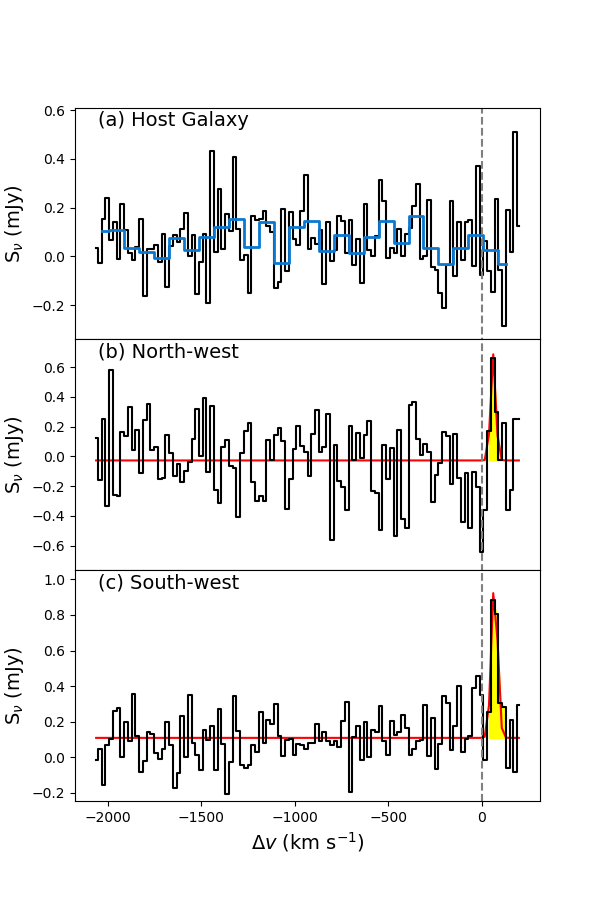
\includegraphics[width=0.6\textwidth, valign=m]{plots_chp4/MRC0943_CI_spectrums.png}}
  \subfloat[]{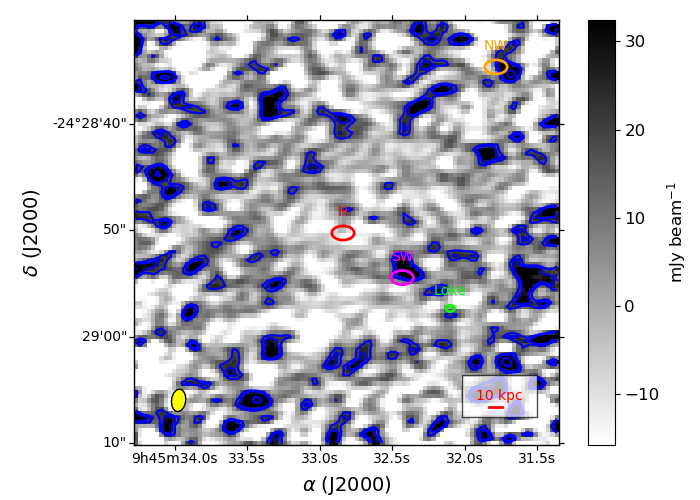
\includegraphics[width=0.65\textwidth, valign=m]{plots_chp4/MRC0943_CI_moment0.png}}
  \caption[{MRC 0943-242 [\ion{C}{i}](1-0) line spectra and moment-0 maps}]{{\it Left:} [\ion{C}{i}](1-0) line emission in {\bf MRC 0943-242}. The spectra are extracted from apertures shown in panel (b) within the regions shown in the [\ion{C}{i}](1-0) moment-0 map. While the channel widths are 20 km s$^{-1}$ for all spectra, an additional spectrum is shown for the host galaxy with 80 km s$^{-1}$ binning in blue. {\it Right:} [\ion{C}{i}](1-0) moment-0 continuum-subtracted map integrated over $\nu_{\rm obs}=125.28-125.38$ GHz. The apertures correspond to the north-west (orange), south-west (pink) and host galaxy (red) with the [\ion{C}{i}](1-0) contours (blue) increasing from $\sigma=18~\rm{mJy~beam}^{-1}.$ The ALMA $2.11\arcsec \times 1.33 \arcsec$ synthesised beam size is shown in yellow. The aperture of the south-west detection from \citet{Gullberg2016a}, named Loke, is shown in green where the synthesized beam is that of $0.7 \arcsec \times 0.8 \arcsec$}
  \label{fig:MRC0943-fit-CI-moment0}
\end{figure*}

\begin{figure*}
\hspace*{-50pt}
\centering
 \subfloat[]{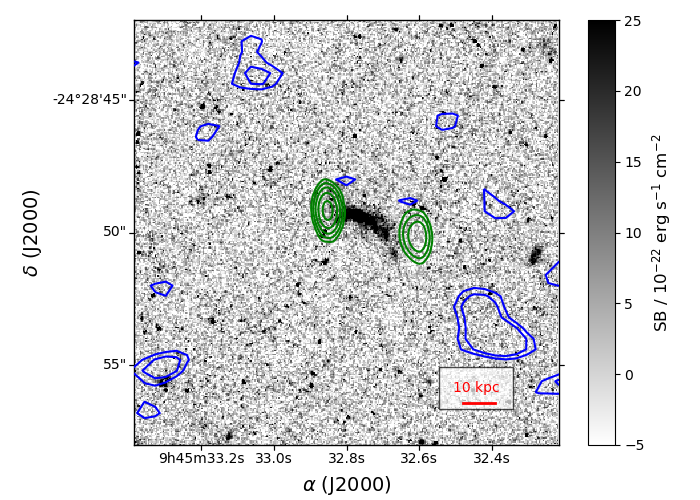
\includegraphics[width=0.6\textwidth]{plots_chp4/MRC0943_hst_CI_VLA_img.png}}
 \subfloat[]{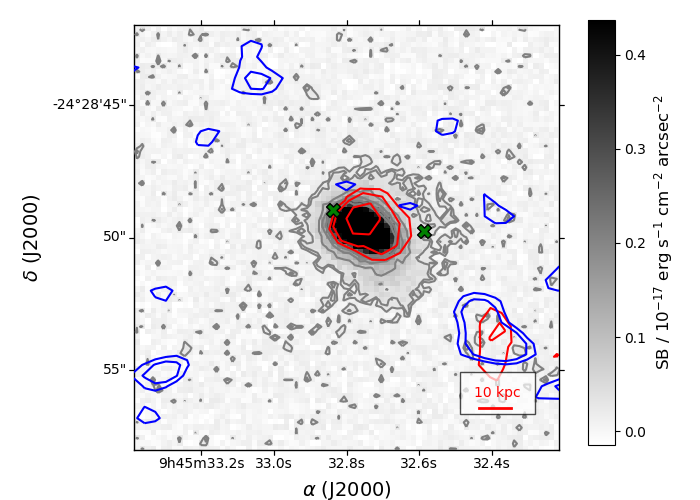
\includegraphics[width=0.6\textwidth]{plots_chp4/USS0943-242_irac2_CI.png}}
 \caption[{MRC 0943-242: [\ion{C}{i}](1-0) moment-0 maps, VLA C-band and Spitzer IRAC 1 images}]{{\it Left:} Map of {\bf MRC 0943-242} similar to Fig. \ref{fig:4C03-hst-irac2-CI-imgs}a with the VLA C-band contours starting at $\sigma=0.4~\rm{mJy~beam}^{-1}.$ {\it Right:} The same [\ion{C}{i}](1-0) contour levels from panel (a) shown over a MUSE pseudo narrow-band image covering $\lambda_{\rm obs}=4732-4800~\ang.$ IRAC 3.6 $\mu$m contours (red) increase from $\sigma=0.05~\rm MJy~sr^{-1}.$ The MUSE contours (grey) increase from $\sigma=0.06 \times 10^{-17}$ erg~s$^{-1}$ \ang$^{-1}$ cm$^{-2}$ pix$^{-1}.$ The green crosses represent the hotspots of the radio lobes determined from the VLA contours.}
  \label{fig:MRC0943-hst-irac2-CI-imgs}
\end{figure*}

\subsection{TN J0205+2422}
% 1 arcsec = 7.485 kpc

We have obtained a redshift of $z=3.5050 \pm 0.0004$ for TN J0205+2422 where the angular scale-size is 7.49 kpc arcsec$^{-1}.$ As Fig. \ref{fig:TNJ0205-fit-CI-moment0}a and \ref{fig:TNJ0205-fit-CI-moment0}b show no [\ion{C}{i}](1-0) line emission is detected at the host galaxy hence we estimate a $3\sigma$ upper limit for the line flux of the host galaxy. Several [\ion{C}{i}](1-0) line detections occur at distances between $d\simeq11.0\arcsec$ and $25.9\arcsec$ ($d\simeq82$ and 194 kpc) to the south-east and east of the host galaxy (see Table \ref{table:alma-line-params1}). 

The [\ion{C}{i}](1-0) lines have widths of $\rm FWHM=33\pm11$ km~s$^{-1}$ in the south-east and $\rm FWHM=39\pm10$ km~s$^{-1}$ in the east, indicating quiescent H$_2$ gas (see Table \ref{table:alma-line-params2}). The imaging in Fig. \ref{fig:TNJ0205-hst-irac2-CI-imgs}a shows a resolved double-lobe radio morphology with a size of $d=21$ kpc that is spatially coincident with the stellar component. Fig. \ref{fig:TNJ0205-hst-irac2-CI-imgs}b shows the giant \lya~emission nebula enshrouding the host galaxy, covering an area of $\sim$82 $\times$ 60 kpc$^2.$ 

We estimate H$_2$ masses at these off-nuclear regions in the order of $M_{\rm H_2}\simeq10^{9}$ M$_\odot$ which is an order of magnitude lower than the $M_{\rm H_2} < 1.6\e{10}$ M$_\odot$ upper limit measured for the host galaxy. The star-formation rate at the host galaxy has an upper limit $\rm SFR < 84~M_\odot yr^{-1}.$ Taking the inferred H$_2$ upper limit into account, we estimate a range of possible depletion time-scales such that $\tau_{\rm depl} < 188$ Myr. 

\begin{figure*}
\hspace*{-50pt}
\centering
\subfloat[]{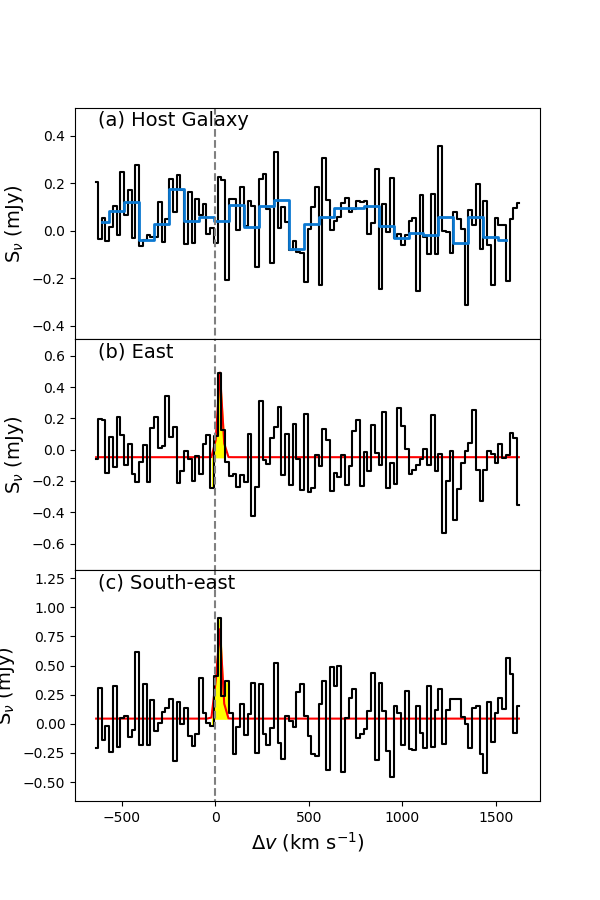
\includegraphics[width=0.6\textwidth, valign=m]{plots_chp4/J0205_CI_spectrums.png}}
\subfloat[]{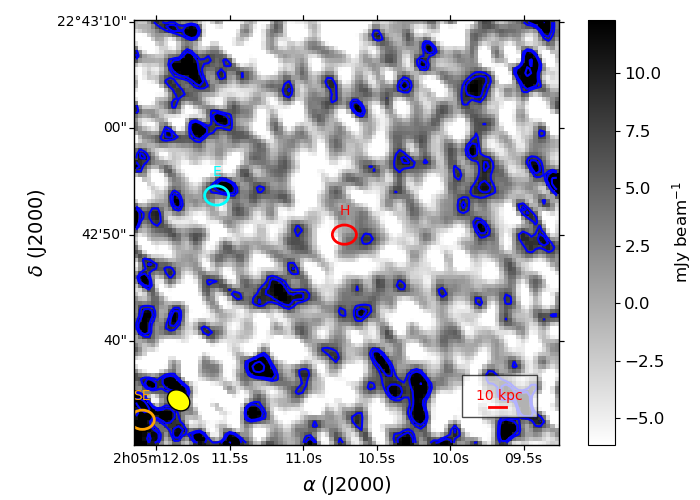
\includegraphics[width=0.65\textwidth, valign=m]{plots_chp4/TN_J0205_CI_moment0.png}}
  \caption[{TN J0205+2422 [\ion{C}{i}](1-0) line spectra and moment-0 maps}]{{\it Left:} [\ion{C}{i}](1-0) line emission in {\bf TN J0205+2422}. The spectra are extracted from apertures shown in panel (b) within the regions shown in the [\ion{C}{i}](1-0) moment-0 map. While the channel widths are 20 km s$^{-1}$ for all spectra, an additional spectrum is shown for the host galaxy with 80 km s$^{-1}$ binning in blue. {\it Right:}  [\ion{C}{i}](1-0) moment-0 continuum-subtracted map integrated over $\nu_{\rm obs}=109.21-109.23$ GHz. The apertures correspond to the north-east (cyan), south-east (orange) and host galaxy (red) with the [\ion{C}{i}](1-0) contours (blue) increasing from $\sigma=5~\rm{mJy~beam}^{-1}.$ The $2.26\arcsec \times 1.81\arcsec$ synthesised beam size is shown in yellow.}
  \label{fig:TNJ0205-fit-CI-moment0}
\end{figure*}

\begin{figure*}
\hspace*{-50pt}
\centering
\subfloat[]{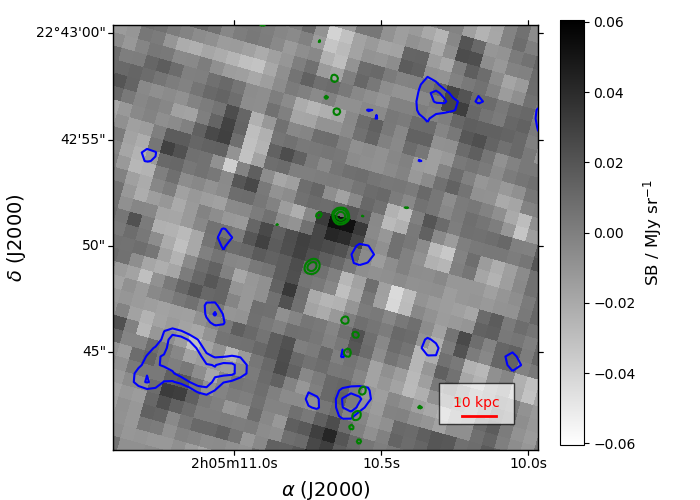
\includegraphics[width=0.6\textwidth]{plots_chp4/TNJ0205_irac_CI_VLA_img.png}}
\subfloat[]{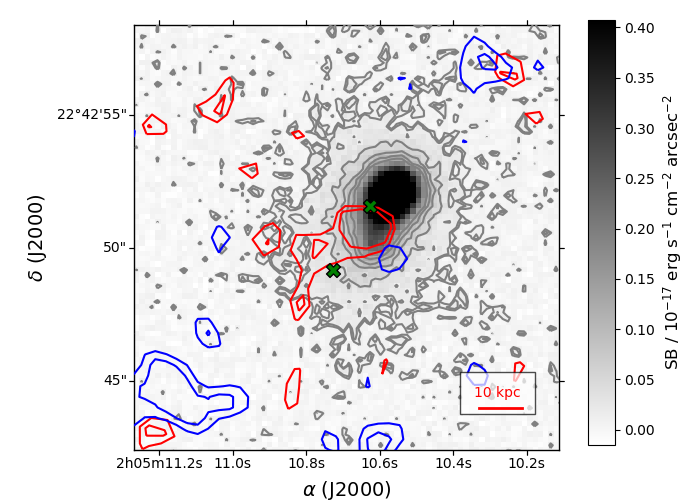
\includegraphics[width=0.6\textwidth]{plots_chp4/TN_J0205+2242_irac2_CI.png}}
  \caption[{TN J0205+2422: [\ion{C}{i}](1-0) moment-0 maps, VLA C-band and Spitzer IRAC 1 images}]{{\it Left:} Map of {\bf TN J0205+2422} similar to Fig. \ref{fig:4C04-hst-irac2-CI-imgs}a with the VLA C-band contours starting at $\sigma=0.08~\rm{mJy~beam}^{-1}.$ {\it Right:} The same [\ion{C}{i}](1-0) contour levels from panel (a) shown over a MUSE pseudo narrow-band image covering $\lambda_{\rm obs}=5452-5500~\ang.$ IRAC 3.6 $\mu$m contours (red) increase from $\sigma=0.02~\rm MJy~sr^{-1}.$ The MUSE contours (grey) increase from $\sigma=0.02 \times 10^{-17}$ erg~s$^{-1}$~\ang$^{-1}$ cm$^{-2}$ pix$^{-1}.$ The green crosses represent the hotspots of the radio lobes determined from the VLA contours.}
  \label{fig:TNJ0205-hst-irac2-CI-imgs}
\end{figure*}

\subsection{TN J0121+1320}\label{section:J0121}
% 1 arcsec = 7.474 kpc

We compute a redshift of $z=3.5181 \pm 0.0003$ for TN J0121+1320 (also catalogued as TXS 0119+130). At this redshift, the angular-size scale is 7.45 kpc arcsec$^{-1}.$ Fig. \ref{fig:TNJ0121-fit-CI-moment0}a and \ref{fig:TNJ0121-fit-CI-moment0}b show [\ion{C}{i}](1-0) line detections at the host galaxy as well as at a projected distances of between $d\simeq24.7\arcsec=185$ kpc to the north-west of the host galaxy (see Table \ref{table:alma-line-params1}). The line-width at the off-nuclear region is $\rm FWHM = 29 \pm 10$ km s$^{-1},$ suggesting dynamically cold gas. The line-width at the host galaxy is broader, in comparison with $\rm FWHM = 157 \pm 40$ km s$^{-1},$ which indicate more turbulent cold gas in the vicinity of the AGN.

The VLA contours in Fig. \ref{fig:TNJ0121-hst-irac2-CI-imgs}a indicate that the radio lobes extend out to $d \simeq 14$ kpc which is evidence of a newly formed radio source. Taking into account the radio size and assuming nominal propagation velocity of $\varv=0.05c,$ we obtain an AGN duty cycle of $\tau_{\rm jet} = 0.91$ Myr which supports the notion that the AGN is relatively young. Fig. \ref{fig:TNJ0121-hst-irac2-CI-imgs}b indicates that the radio hotspot spatially coincides with the stellar emission. Hence, the jets are clearly associated with the host galaxy. The \lya~emission nebula extends over an area of $\sim$26 $\times$ 19 kpc$^2.$ The surface brightness peak of the \lya~emission, however, is slightly offset to the south-east.  

The [\ion{C}{i}](1-0) line emission in the north-west implies an H$_2$ mass of $\rm M_{\rm H_2} = (6.0 \pm 2.2)\e{10}$ M$_\odot.$ At the host galaxy, an H$_2$ mass inferred is $\rm M_{\rm H_2} = (1.0 \pm 0.1)\e{10}$ M$_\odot$ (see Table \ref{table:alma-line-params2}). The host galaxy has a relatively high star-formation rate of $\rm SFR=626$ M$_\odot$ yr$^{-1},$ which leads to a depletion time-scale of $\tau_{\rm depl} = 17$ Myr. CO(4-3) line detections in this source were reported in \citet{deBreuck2003}. The measure of $S_{\rm CO(4-3)}\rm dV=1.2\pm0.4$ Jy km~s$^{-1},$ which corresponds to a CO(4-3) luminosity of $\rm L'_{\rm CO(4-3)} = (1.97 \pm 0.66)\e{9}$ K km s$^{-1}$ pc$^2$. 

\begin{figure*}
\hspace*{-50pt}
\centering
\subfloat[]{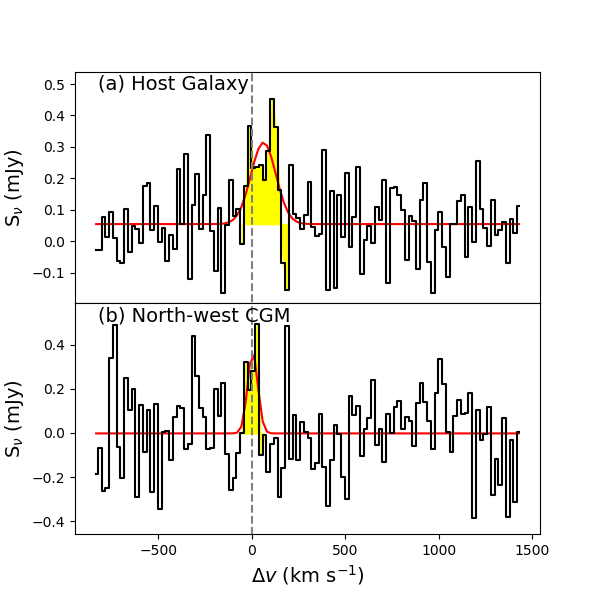
\includegraphics[width=0.6\textwidth, valign=m]{plots_chp4/J0121_CI_spectrums.png}}
\subfloat[]{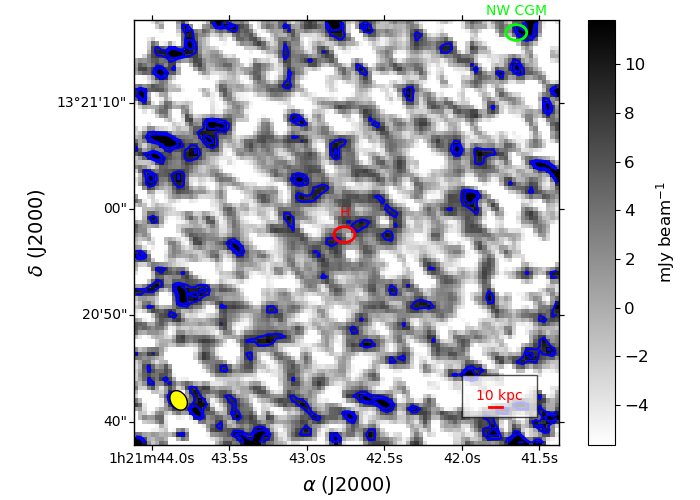
\includegraphics[width=0.65\textwidth, valign=m]{plots_chp4/TN_J0121_CI_moment0.png}}
  \caption[{TN J0121+1320 [\ion{C}{i}](1-0) line spectra and moment-0 maps}]{{\it Left:} [\ion{C}{i}](1-0) line emission in {\bf TN J0121+1320}. The spectra are extracted from apertures shown in panel (b) within the regions shown in the [\ion{C}{i}](1-0) moment-0 map. {\it Right:} [\ion{C}{i}](1-0) moment-0 continuum-subtracted map integrated over $\nu_{\rm obs}=108.81-108.93$ GHz. The apertures correspond to the north-west CGM (green) and host galaxy (red) with the [\ion{C}{i}](1-0) contours (blue) increasing from $\sigma=8~\rm{mJy~beam}^{-1}.$ The $1.97\arcsec \times 1.48\arcsec$ synthesised beam size is shown in yellow.}
  \label{fig:TNJ0121-fit-CI-moment0}
\end{figure*}

\begin{figure*}
\hspace*{-50pt}
\centering
\subfloat[]{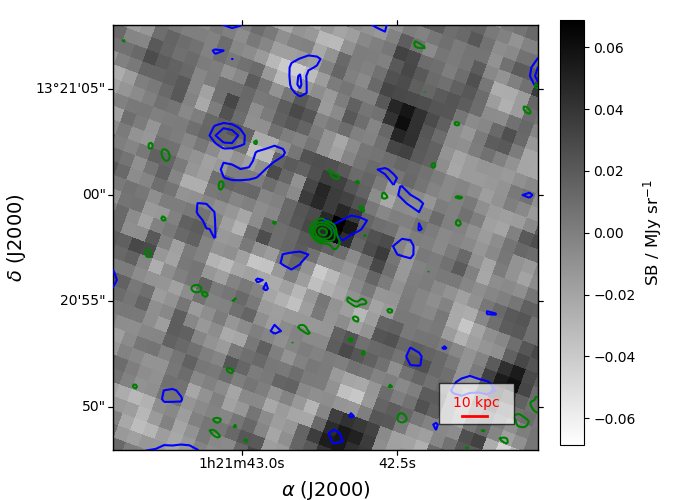
\includegraphics[width=0.6\textwidth]{plots_chp4/TN_J0121_irac_CI_VLA_img.png}}
\subfloat[]{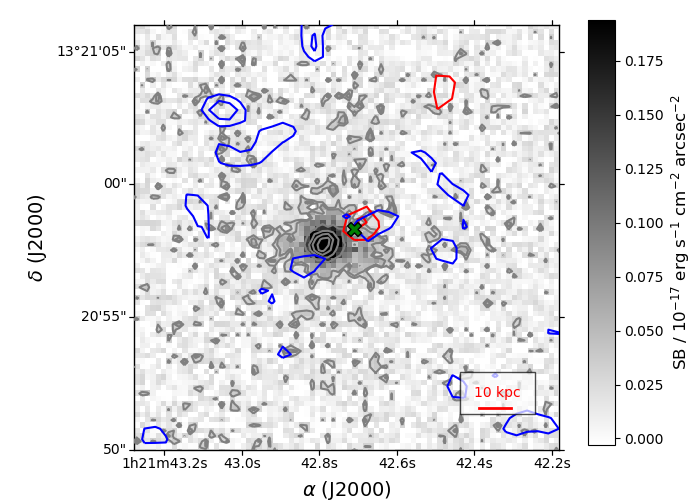
\includegraphics[width=0.6\textwidth]{plots_chp4/TN_J0121+1320_irac2_CI.png}}
\caption[{TN J0121+1320: [\ion{C}{i}](1-0) moment-0 maps, VLA C-band and Spitzer IRAC 1 images}]{{\it Left:} Map of {\bf TN J0121+1320} similar to Fig. \ref{fig:4C04-hst-irac2-CI-imgs}a with the VLA C-band contours starting at $\sigma=0.2~\rm{mJy~beam}^{-1}.$ {\it Right:} The same [\ion{C}{i}](1-0) contour levels from panel (a) shown over a MUSE pseudo narrow-band image covering $\lambda_{\rm obs}=5471-5525~\ang.$ IRAC 3.6 $\mu$m contours (red) increase from $\sigma=0.05~\rm MJy~sr^{-1}.$ The MUSE contours (grey) increase from $\sigma=0.08 \times 10^{-17}$ erg~s$^{-1}$ \ang$^{-1}$ cm$^{-2}$ pix$^{-1}.$ The green crosses represent the hotspots of the radio lobes determined from the VLA contours.}
  \label{fig:TNJ0121-hst-irac2-CI-imgs}
\end{figure*}

\subsection{4C+03.24}\label{section:4C03}
% 1arcsec = 7.437 kpc 

The systemic redshift we obtain for 4C+03.24 is $z=3.5650 \pm 0.0006$ at which the angular-size scale is 7.44 kpc arcsec$^{-1}.$ Figs \ref{fig:4C03-fit-CI-moment0}a and \ref{fig:4C03-fit-CI-moment0}b show line detections at two off-nuclear regions. A [\ion{C}{i}](1-0) detection is made $d \simeq 2.03 \arcsec=15$ kpc to the north-east of the galaxy and another at $d \simeq 15.03 \arcsec = 112$ kpc from the host galaxy centre. At the host galaxy, where no [\ion{C}{i}](1-0) line emission is detected, we estimate a $3\sigma$ upper limit for the [\ion{C}{i}](1-0) flux. The line-widths for the [\ion{C}{i}](1-0) emission in the north and east are $\rm FWHM=50\pm18$ km s$^{-1}$ and $\rm FWHM=65\pm29$ km s$^{-1}$ (see Table \ref{table:alma-line-params1}). 

The radio lobes have a resolved double morphology and extend to $d\simeq55$ kpc which \citet{vanojik1996} describe as an asymmetric morphology that may mean that the jet has been deflected by a dense region in the gas halo. The narrow-band imaging in Fig. \ref{fig:4C03-hst-irac2-CI-imgs}a shows that the dominant [\ion{C}{i}](1-0) line emission coincides partially with the northern radio lobe. We also show a \lya~narrow-band of the galaxy in Fig. \ref{fig:4C03-hst-irac2-CI-imgs}b, over the wavelength range selected and spans an area of $\sim$37 $\times$ 18 kpc$^2.$ Additionally, the diffuse, low surface-brightness component (or outer halo) extends to $d\simeq90$ kpc from the nucleus \citep{Gopal-Krishna2000}. The IRAC 3.6 $\mu$m contours in this figure, coincide spatially with the [\ion{C}{i}](1-0) line emission. 

The jet deflection-zone is also where the surface brightness of \lya~emission is enhanced as well as blueshifted by $\Delta \varv \simeq -1100$ km s$^{-1}.$ Additionally, radio polarisation maps show a high level of depolarisation in the northern jet relative to the southern one implying that the deflected jet is approaching. Our results are consistent with {\it Subaru} observations from \citet{Ohyama2004} which show turbulent kinematics within the inner regions of the \lya~halo. This is indicated by line-widths of $\rm FWHM \simeq 1900$ km s$^{-1},$ and velocity shifts of $\Delta \varv \simeq -1000$ km s$^{-1}.$ 

The masses of H$_2$ measured are M$_{\rm H_2} = (4.9 \pm 1.1)\e{9}$ M$_\odot$ in the north and M$_{\rm H_2} = (6.8 \pm 1.5)\e{10}$ M$_\odot$ in the east region. The host galaxy H$_2$ mass has an upper limit of M$_{\rm H_2} < 1.3\e{10}$ M$_\odot$ (see Table \ref{table:alma-line-params2}). A star-formation rate, $\rm SFR = 142$ M$_\odot$ yr$^{-1}$ at the host galaxy implies that the molecular gas will deplete in $\tau_{\rm depl} < 93$ Myr.  

\begin{figure*}
\hspace*{-50pt}
\centering
	\subfloat[]{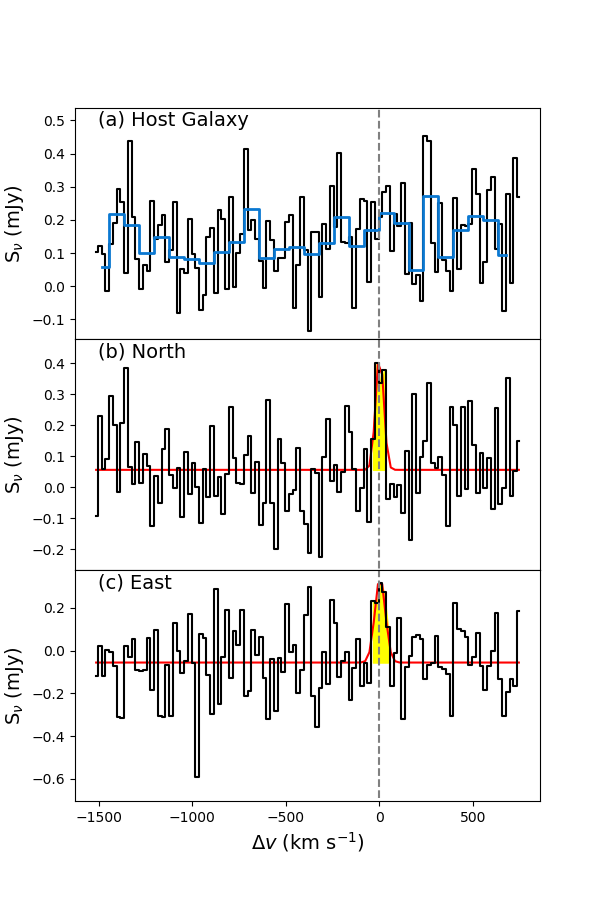
\includegraphics[width=0.6\textwidth, valign=m]{plots_chp4/4C03_CI_spectrums.png}}
	\subfloat[]{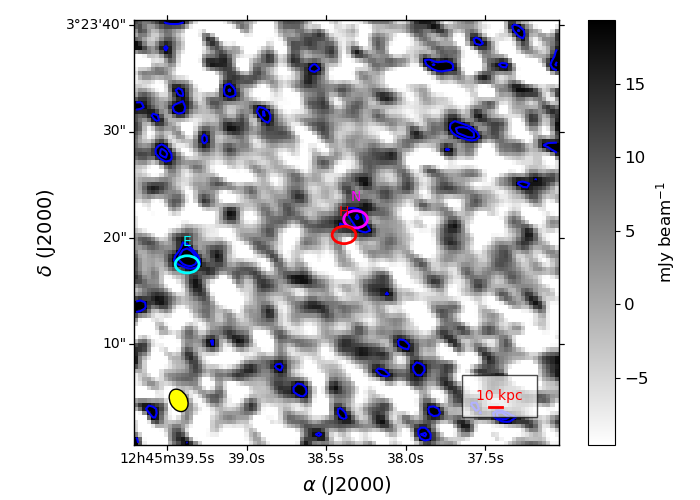
\includegraphics[width=0.65\textwidth, valign=m]{plots_chp4/4C03_CI_moment0.png}}
\caption[{4C+03.24 [\ion{C}{i}](1-0) line spectra and moment-0 maps}]{{\it Left:} [\ion{C}{i}](1-0) line emission in {\bf 4C+03.24} spectra extracted from the apertures shown in panel (b). The detections are highlighted in yellow, hence the host galaxy has a [\ion{C}{i}](1-0) non-detection. While the channel widths are 20 km s$^{-1}$ for all spectra, an additional spectrum is shown for the host galaxy with 80 km s$^{-1}$ binning in blue. {\it Right:} [\ion{C}{i}](1-0) moment-0 continuum-subtracted map integrated over $\nu_{\rm obs}=107.75 - 107.86$ GHz. The apertures shown represent the north-west (magenta), east (cyan) and host galaxy (red) regions. The $n$th [\ion{C}{i}](1-0) contour (blue) occurs at a surface brightness level of $\sqrt{2}{n}\sigma$ for $n$ increases in unity increments and $\sigma = 18~\rm{mJy~beam}^{-1}.$ The $2.23\arcsec \times 1.62\arcsec$ synthesised beam is represented in yellow. }
\label{fig:4C03-fit-CI-moment0}
\end{figure*}

\begin{figure*}
\hspace*{-50pt}
\centering
	\subfloat[]{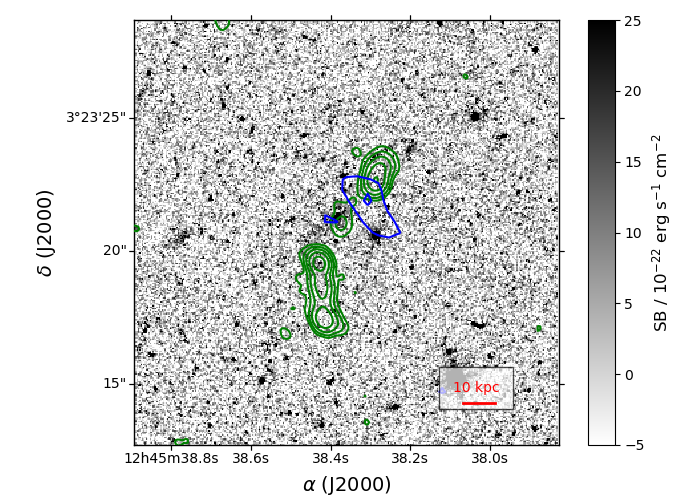
\includegraphics[width=0.6\textwidth]{./plots_chp4/4C03_hst_CI_VLA_img.png}}
	\subfloat[]{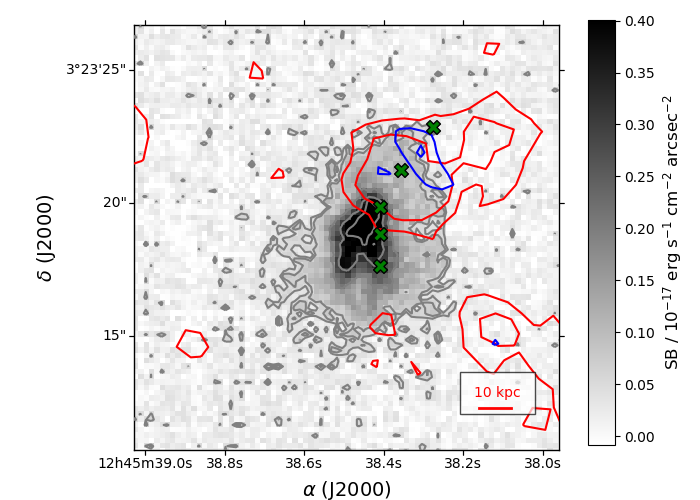
\includegraphics[width=0.6\textwidth]{./plots_chp4/USS1243+036_irac2_CI.png}}
\caption[{4C+03.24: [\ion{C}{i}](1-0) moment-0 maps, VLA C-band and Spitzer IRAC 1 images}]{{\it Left:} [\ion{C}{i}](1-0) line emission in {\bf 4C+03.24} is shown in contours (blue) against VLA C-band (radio) detections tracing the radio lobes that extend out to $d\simeq55$ kpc. The $n$th radio contour (green) occurs at a surface brightness level of $(2\sqrt{2})^n\sigma$ for which $\sigma = 0.16~\rm{mJy~beam}^{-1}.$ {\it Right:} [\ion{C}{i}](1-0) emission also coincides with the surface-brightness peak in the HST WFPC2 702W tracing the UV/optical continuum ($\lambda_{\rm obs}=5800-8600~\ang$). The Spitzer/IRAC 1 (3.6 $\mu$m) detections, which trace the stellar distribution, coincide spatially with [\ion{C}{i}](1-0) line emission. The IRAC contours increase as $(2\sqrt{2})^n\sigma$ for $\sigma=0.06~\rm MJy~sr^{-1}.$ The image shows a MUSE narrow-band \lya~image that has been integrated over a wavelength range of $\lambda_{\rm obs}=5532- 5586~\ang.$ The $n$th MUSE contour (grey) occurs at surface brightness level of $\sqrt{2}n\sigma$ for $n$ increasing in increments of 2 and $\sigma = 0.1\times 10^{-17}$ erg~s$^{-1}$ \ang$^{-1}$ cm$^{-2}$ pix$^{-1}.$ The green crosses represent the hotspots of the radio lobes determined from the VLA contours.}
    \label{fig:4C03-hst-irac2-CI-imgs}
\end{figure*} 

\subsection{4C 19.71}
% 1 arcsec = 7.418 kpc

We have computed a redshift of $z=3.5892 \pm 0.0003$ for 4C19.71 (also known as MG 2144+1928). At this redshift, the angular-size scale is 7.42 kpc arcsec$^{-1}.$ Fig. \ref{fig:4C19-fit-CI-moment0}a and \ref{fig:4C19-fit-CI-moment0}b show that [\ion{C}{i}](1-0) emission is not detected at the host galaxy and we obtain a $3\sigma$ upper limit. Two off-nuclear [\ion{C}{i}](1-0) detections are obtained to the south-east (at $d\simeq2\arcsec=18$ kpc) as well as to north-west (at $d\simeq18\arcsec=133$ kpc) of the host galaxy. The line-widths are $\rm FWHM = 33\pm14$ km s$^{-1}$ and $\rm FWHM = 33\pm14$ km s$^{-1}$ in the north-west and south-east indicating quiescent gas in extended gas halo or CGM (see Table \ref{table:alma-line-params1}). 

The VLA contours in Fig. \ref{fig:4C19-hst-irac2-CI-imgs}a show a double-lobe morphology of extent $d\simeq133$ kpc. Coincidentally, the \lya~emission nebula shown in Fig. \ref{fig:4C19-hst-irac2-CI-imgs}b has an elongated morphology in the N-S direction which is in alignment with the radio axis and spans an area of $\sim$119$\times$44 kpc$^2.$ The south-east [\ion{C}{i}](1-0) detection is located within the expanse of the \lya~emission nebula and coincides spatially with one of two stellar components. 

At the off-nuclear regions, we obtain H$_2$ masses of M$_{\rm H_2} = (4.7\pm1.5)\e{9}$ M$_\odot$ in the south-east and M$_{\rm H_2} = (4.5\pm1.6)\e{9}$ M$_\odot$ in the north-west. The H$_2$ host galaxy gas mass estimated is M$_{\rm H_2}<1.7\e{10}$ M$_\odot$ (see Table \ref{table:alma-line-params2}). The host galaxy has a star-formation rate of $\rm SFR = 84~M_\odot$ yr$^{-1}$ which implies a depletion of H$_2$ gas over a period of $\tau_{\rm depl} < 199$ Myr. 

These findings are consistent with those of \citet{falkendal2019-submitted} who also use [\ion{C}{i}](1-0) to trace H$_2.$ They also find that this gas is quiescent with line-widths of $\rm FWHM\simeq 100$ km s$^{-1}$ at $d\sim75$ kpc from the nucleus of the host galaxy. Following up their findings with a basic photoionisation model from \pkg{cloudy} \citep{Ferland2013}, they estimate a low metallicity for the gas of  $\rm 0.03 < Z/Z_\odot < 0.1.$ 

\begin{figure*}
\hspace*{-50pt}
\centering
\subfloat[]{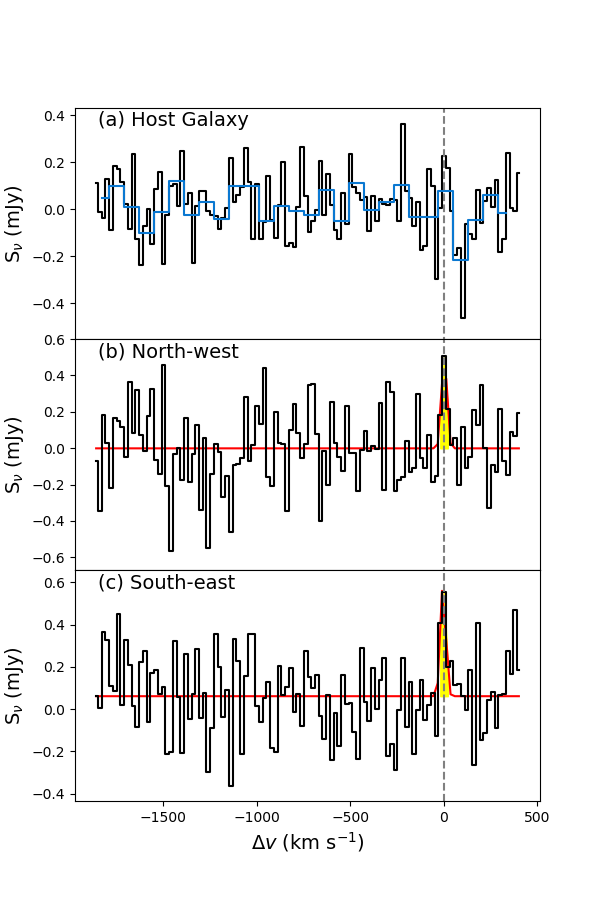
\includegraphics[width=0.6\textwidth, valign=m]{plots_chp4/4C19_CI_spectrums.png}}
\subfloat[]{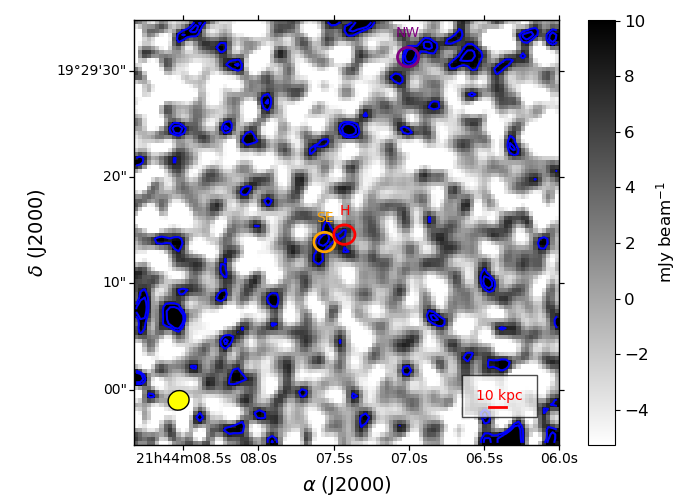
\includegraphics[width=0.65\textwidth, valign=m]{plots_chp4/4C19_CI_moment0.png}}
  \caption[{4C 19.71 [\ion{C}{i}](1-0) line spectra and moment-0 maps}]{{\it Left:} [\ion{C}{i}](1-0) line emission in {\bf 4C 19.71}. The spectra are extracted from apertures shown in panel (b) within the regions shown in the [\ion{C}{i}](1-0) moment-0 map. While the channel widths are 20 km s$^{-1}$ for all spectra, an additional spectrum is shown for the host galaxy with 80 km s$^{-1}$ binning in blue. {\it Right:} [\ion{C}{i}](1-0) moment-0 continuum-subtracted map integrated over $\nu_{\rm obs}=107.241-107.243$ GHz. The apertures correspond to the north-west CGM (purple), south-east (orange) and host galaxy (red) with the [\ion{C}{i}](1-0) contours (blue) increasing from $\sigma=8~\rm{mJy~beam}^{-1}.$ The $1.99\arcsec \times 1.82\arcsec$ synthesised beam size is shown (yellow).}
  \label{fig:4C19-fit-CI-moment0}
\end{figure*}

\begin{figure*}
\hspace*{-50pt}
\centering
\subfloat[]{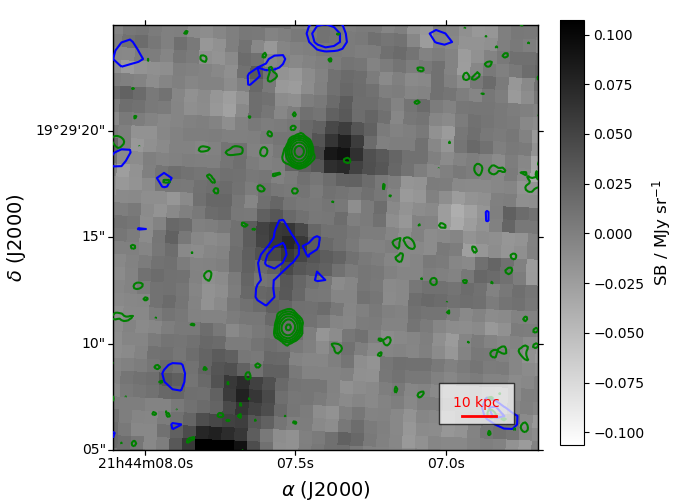
\includegraphics[width=0.6\textwidth]{plots_chp4/4C19_irac_CI_VLA_img.png}}
\subfloat[]{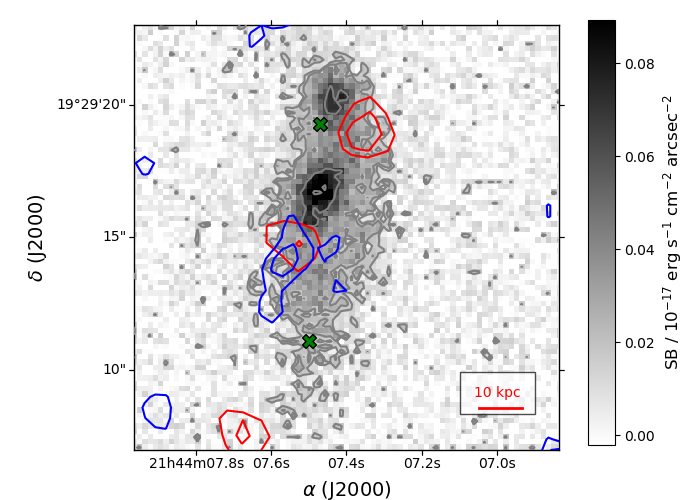
\includegraphics[width=0.6\textwidth]{plots_chp4/MG_2144+1928_irac2_CI.png}}
\caption[{4C 19.71: [\ion{C}{i}](1-0) moment-0 maps, VLA C-band and Spitzer IRAC 1 images}]{{\it Left:} Map of {\bf 4C 19.71} similar to Fig. \ref{fig:4C04-hst-irac2-CI-imgs}a with the VLA C-band contours starting at $\sigma=0.1~mJy.$ {\it Right:} The same [\ion{C}{i}](1-0) contour levels from panel (a) shown over a MUSE pseudo narrow-band image covering $\lambda_{\rm obs}=5560-5608~\ang.$ IRAC 3.6 $\mu$m contours (red) increase from $\sigma=0.05~\rm MJy~sr^{-1}.$ The MUSE contours (grey) increase from $\sigma=0.03 \times 10^{-17}$ erg~s$^{-1}$ \ang$^{-1}$ cm$^{-2}$ pix$^{-1}.$ The green crosses represent the hotspots of the radio lobes determined from the VLA contours.}
  \label{fig:4C19-hst-irac2-CI-imgs}
\end{figure*}

\subsection{TN J1338-1942}
% 1 arcsec =  7.021 kpc

The redshift of TN J1338-1942 obtained here is $z=4.1077 \pm 0.0024,$ where the angular-size scale is 7.02 kpc arcsec$^{-1}.$ Fig. \ref{fig:TNJ1338-fit-CI-moment0}a and \ref{fig:TNJ1338-fit-CI-moment0}b demonstrate that no [\ion{C}{i}](1-0) emission is detected at the host galaxy but rather an upper limit is obtained. Four detections lie between distances of $d\simeq16.06\arcsec$ and $19.51\arcsec$ ($d\simeq113$ and 137 kpc) from the host galaxy (see Table \ref{table:alma-line-params1}). Their distances from the nucleus imply that the gas being traced lies within the CGM rather than the ISM of the galaxy. 

The VLA contours in Fig. \ref{fig:TNJ1338-hst-irac2-CI-imgs}a do not have a clearly defined double-lobe morphology, showing that the radio lobes extend to $d \sim10$ kpc, which implies a jet age, $\tau_{\rm jet} = 0.65$ Myr. This duty cycle and radio size imply a freshly ignited AGN. The contours reveal only one radio hotspot which makes this source similar to TN J0121+1320 with the main difference being that its \lya~emission nebula is far more extended. Fig. \ref{fig:TNJ1338-hst-irac2-CI-imgs}b shows that the stellar emission spatially coincides with the surface brightness peak within the \lya~halo as well as the source's radio hotspot. In the image, the \lya~halo extends to $\sim$126 $\times$ 63 kpc$^2,$ which is rather consistent with the 150 $\times$ 80 kpc$^2$ from \citet{swinbank2015}. 

The H$_2$ masses of the four tentative detections are all approximately of the order of M$_{\rm H_2} \simeq 10^{9}$ M$_\odot.$ At the host galaxy, we obtain a upper limit for the H$_2$ mass of M$_{\rm H_2} < 1.4\e{10}$ M$_\odot.$ The star-formation rate of this source is $\rm SFR = 461$ M$_\odot$ yr$^{-1}$ which leads to relatively rapid depletion time-scale of $\tau_{\rm depl}<11$ Myr (see Table \ref{table:alma-line-params2}). 

\begin{figure*}
\vspace*{-20pt}
\hspace*{-50pt}
\centering
\subfloat[]{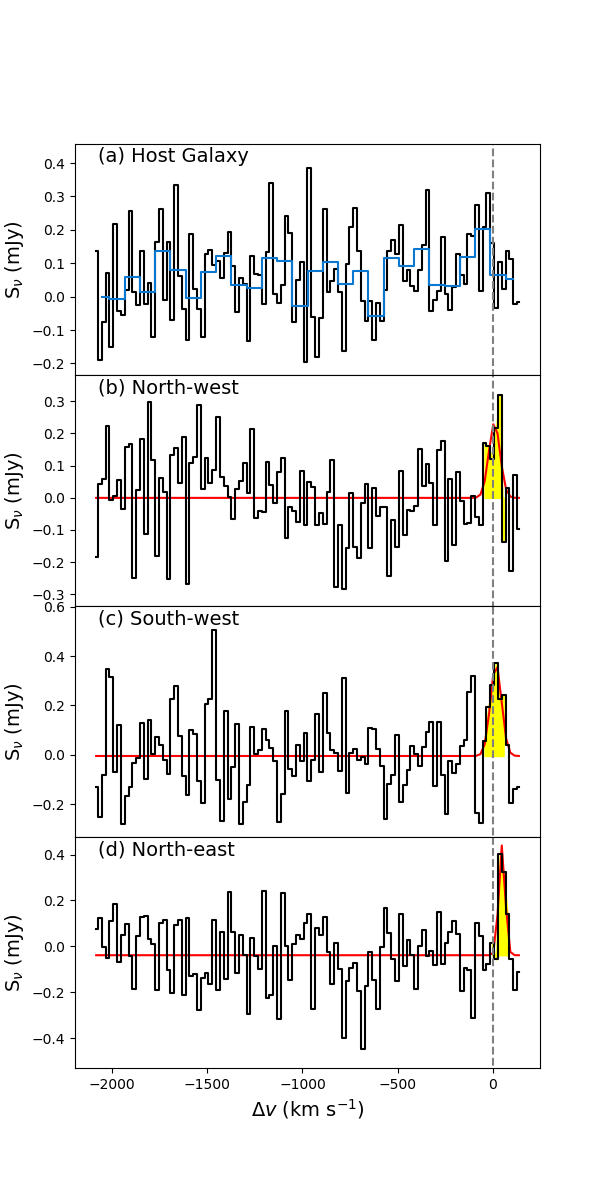
\includegraphics[width=0.6\textwidth, valign=m]{plots_chp4/J1338_CI_spectrums.png}}
\subfloat[]{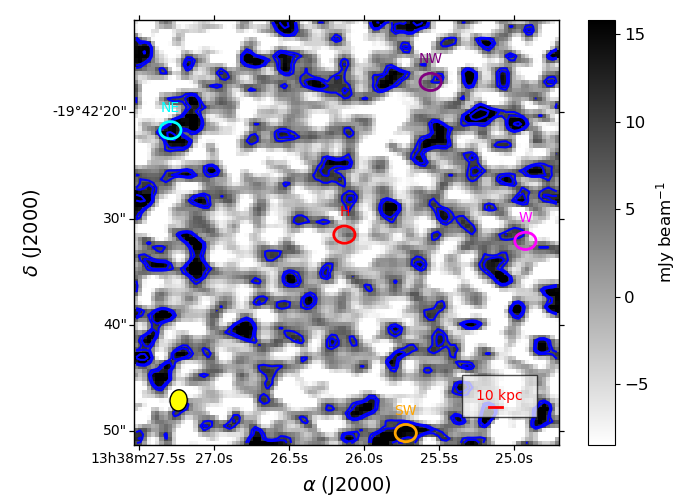
\includegraphics[width=0.65\textwidth, valign=m]{plots_chp4/TNJ1338_CI_moment0.png}}
  \caption[{TN J1338-1942: [\ion{C}{i}](1-0) line spectra and moment-0 maps}]{{\it Left:} [\ion{C}{i}](1-0) line emission in {\bf TN J1338-1942}. The spectra are extracted from apertures shown in panel (b) within the regions shown in the [\ion{C}{i}](1-0) moment-0 map. While the channel widths are 20 km s$^{-1}$ for all spectra, an additional spectrum is shown for the host galaxy with 80 km s$^{-1}$ binning in blue. {\it Right:} [\ion{C}{i}](1-0) moment-0 continuum-subtracted map integrated over $\nu_{\rm obs}=96.23-96.33$ GHz. The apertures correspond to the north-west CGM (purple), north-east (cyan), west (magenta), south-west (orange) and host galaxy (red) with the [\ion{C}{i}](1-0) contours (blue) increasing from $\sigma=8~\rm{mJy~beam}^{-1}.$ The $2.00\arcsec \times 1.62\arcsec$ synthesised beam size is shown in yellow.}
  \label{fig:TNJ1338-fit-CI-moment0}
\end{figure*}

\begin{figure*}
\hspace*{-50pt}
\centering
\subfloat[]{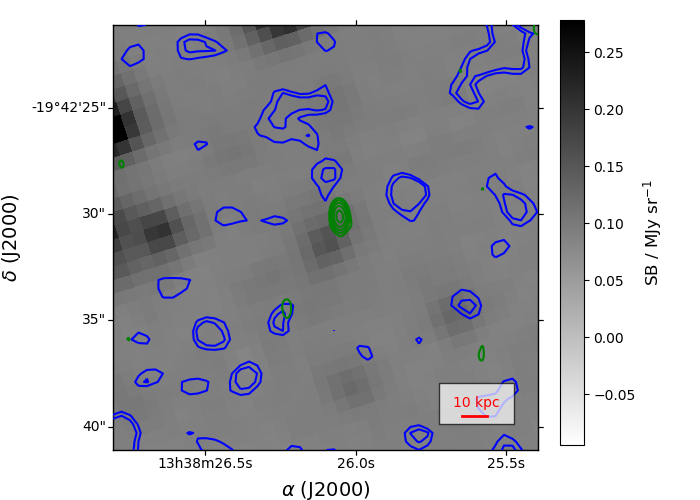
\includegraphics[width=0.6\textwidth]{plots_chp4/TNJ1338_irac_CI_VLA_img.png}}
\subfloat[]{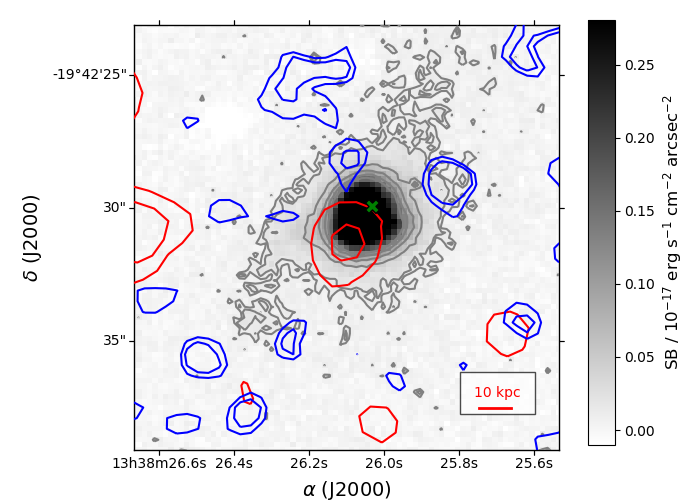
\includegraphics[width=0.6\textwidth]{plots_chp4/TN_J1338-1942_irac2_CI.png}}
\caption[{TN 1338-1942: [\ion{C}{i}](1-0) moment-0 maps, VLA C-band and Spitzer IRAC 1 images}]{{\it Left:} Map of {\bf TN 1338-1942} similar to Fig. \ref{fig:4C04-hst-irac2-CI-imgs}a with the VLA C-band contours starting at $\sigma=0.2~\rm{mJy~beam}^{-1}.$ {\it Right:} The same [\ion{C}{i}](1-0) contour levels from panel (a) shown over a MUSE pseudo narrow-band image covering $\lambda_{\rm obs}=6170-6236~\ang.$ IRAC 3.6 $\mu$m contours (red) increase from $\sigma=0.02~\rm MJy~sr^{-1}.$ The MUSE contours (grey) increase from $\sigma=0.03 \times 10^{-17}$ erg~s$^{-1}$ \ang$^{-1}$ cm$^{-2}$ pix$^{-1}.$ The green crosses represent the hotspots of the radio lobes determined from the VLA contours.}
  \label{fig:TNJ1338-hst-irac2-CI-imgs}
\end{figure*}

\subsection{4C+04.11}\label{section:4C04}
% 1 arcsec = 6.732 kpc

The redshift of the host galaxy 4C+04.11 (also catalogued as RC J0311+0507) we compute is $z=4.5082 \pm 0.0003.$ At this redshift, the angular-size scale is 6.73 kpc arcsec$^{-1}.$ In Figs \ref{fig:4C04-fit-CI-moment0}a and \ref{fig:4C04-fit-CI-moment0}b, we show a [\ion{C}{i}](1-0) detection of $d\simeq14.62\arcsec = 98$ kpc at the host galaxy. No [\ion{C}{i}](1-0) line emission is detected at the host galaxy and instead we obtain a $3\sigma$ upper limit (see Table \ref{table:alma-line-params1}). 

The radio lobes shown in Fig. \ref{fig:4C04-hst-irac2-CI-imgs}a show a morphology that extends to $d\simeq20$ kpc. We estimate the age of the radio jet by assuming a nominal radio lobe propagation speed of $\varv \simeq0.05c$ which together with its radio size, implies that the AGN duty cycle is $\tau_{\rm jet}\simeq1.3$ Myr, consistent with the $\sim$1 Gyr radio source age obtained by \citet{Parijskij2014}.

The \lya~halo spans an area of $\sim$77 $\times$ 36 kpc$^2,$ extending well beyond the southern lobe but does not coincide spatially with the northern hotspot of the radio jets as Fig. \ref{fig:4C04-hst-irac2-CI-imgs}b illustrates. The H$_2$ mass estimate for the north-east detection is M$_{\rm H_2}=(5.9\pm1.2)\e{9}$ M$_\odot.$ At the host galaxy, we obtain an upper limit of M$_{\rm H_2} < 2.2\e{10}$ M$_\odot$ (see Table \ref{table:alma-line-params2}). There is no formal SFR estimate from for this source. Given that it has the highest redshift within the sample. This is a relatively young radio source, and the highest H$_2$ mass upper limit of the galaxies sampled. This may be a result of star-formation having yet to begin depleting the gas. 

\begin{figure*}
\hspace*{-50pt}
\centering
	\subfloat[]{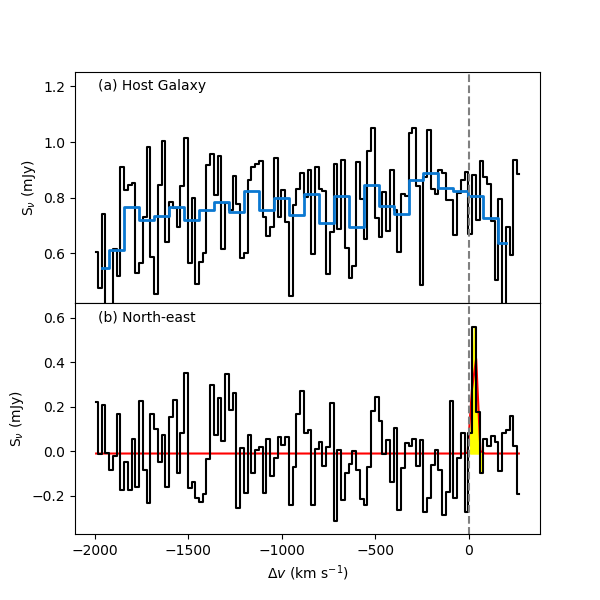
\includegraphics[width=0.6\textwidth, valign=m]{plots_chp4/4C04_CI_spectrums.png}}
	\subfloat[]{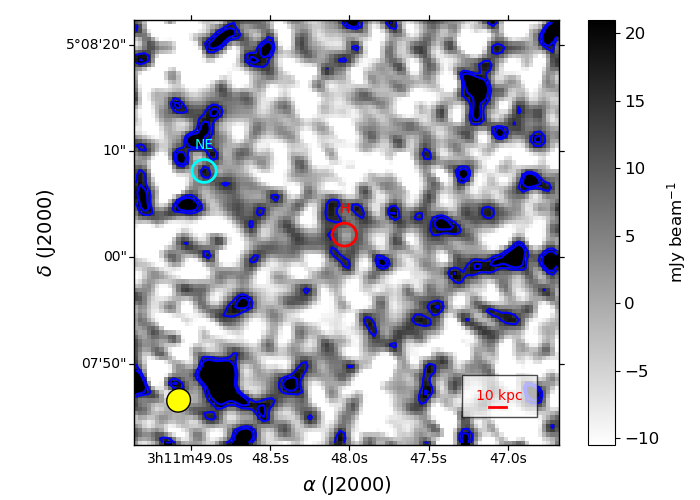
\includegraphics[width=0.65\textwidth, valign=m]{./plots_chp4/4C04_CI_moment0.png}}
\caption[{4C+04.11 [\ion{C}{i}](1-0) line spectra and moment-0 maps}]{{\it Left:} [\ion{C}{i}](1-0) line emission in {\bf 4C+04.11}. The spectra are extracted from apertures shown in panel (b) within the regions shown in the [\ion{C}{i}](1-0) moment-0 map. While the channel widths are 20 km s$^{-1}$ for all spectra, an additional spectrum is shown for the host galaxy with 80 km s$^{-1}$ binning in blue. {\it Right:} [\ion{C}{i}](1-0) moment-0 continuum-subtracted map integrated over $\nu_{\rm obs}=89.25 - 89.37$ GHz. The apertures correspond to the north-east (cyan) and host galaxy (red) regions with the [\ion{C}{i}](1-0) contours (blue) increasing from $\sigma = 14~\rm{mJy~beam}^{-1}.$ The $2.27\arcsec \times 2.16\arcsec$ synthesised beam size is shown in yellow.}
\label{fig:4C04-fit-CI-moment0}
\end{figure*}

\begin{figure*}
\hspace*{-50pt}
\centering 
  \subfloat[]{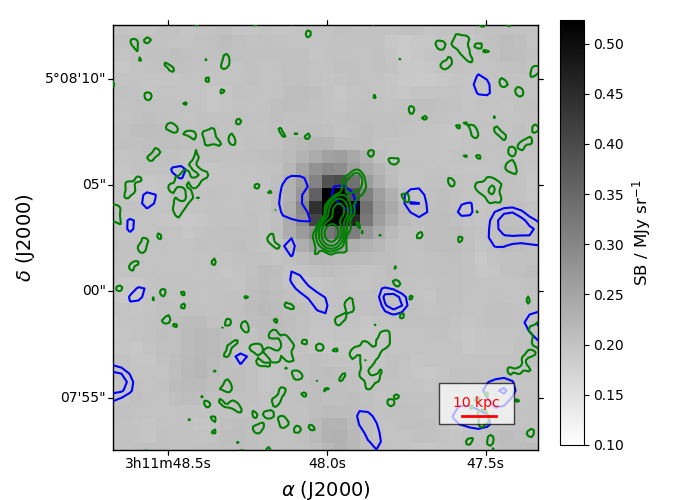
\includegraphics[width=0.6\textwidth]{plots_chp4/4C04_irac_CI_VLA_img.png}}
  \subfloat[]{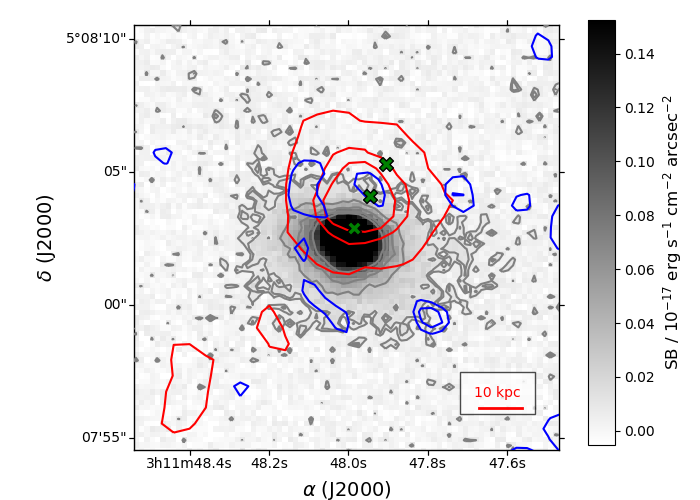
\includegraphics[width=0.6\textwidth]{plots_chp4/4C04+11_irac2_CI.png}}
  \caption[{4C+04.11: [\ion{C}{i}](1-0) moment-0 maps, VLA C-band and Spitzer IRAC 1 images}]{{\it Left:} [\ion{C}{i}](1-0) line emission in {\bf 4C+04.11} is shown in contours (blue) over an IRAC 1 (3.6 $\mu$m) image. The VLA C-band contours (green) increase from $\sigma = 0.4~\rm{mJy~beam}^{-1}.$ {\it Right:} Identical [\ion{C}{i}](1-0) contour levels as panel (a) are shown over a MUSE narrow-band image, integrated over the range, $\lambda_{\rm obs}=6677 - 6739~\ang,$ showing the extent of the \lya~halo. The IRAC 1 contours (red) increase similar to the VLA contours from $\sigma=0.05~\rm MJy~sr^{-1}.$ The MUSE contours (grey) increase from $\sigma=0.02 \times 10^{-17}$ erg~s$^{-1}$ \ang$^{-1}$ cm$^{-2}$ pix$^{-1}.$ The green crosses represent the hotspots of the radio lobes determined from the VLA contours.}
  \label{fig:4C04-hst-irac2-CI-imgs}
\end{figure*}

\begin{sidewaystable*}
	\centering
	\caption[{Observed ALMA [\ion{C}{i}](1-0) line parameters}]{ALMA [\ion{C}{i}](1-0) line parameters. Column (1) is the catalogue name of the galaxy. Column (2) gives the redshift, and column (3) specifies the region name assigned to the location for the detection. Column (4) is the observed frequency, column (5) is the velocity shift which is $\Delta \varv = \varv_{[\rm CI]}  - \varv_{\rm sys.}$ i.e. the [\ion{C}{i}](1-0) line emission velocity shift from the systemic velocity ($\varv_{\rm sys}$). Column (6) is the full-width half maximum (FWHM) of the line, and column (7) is the integrated flux. For non-detections, $3\sigma$ upper flux upper limits are reported assuming a line-width of 100 km s$^{-1}.$ }
	\label{table:alma-line-params1}
	\begin{tabular}{l D{,}{\, \,\pm\, \,}{5} l D{,}{\, \,\pm\, \,}{-6} D{,}{\, \,\pm\, \,}{-6} D{,}{\,\,\pm\,\,}{0} D{,}{\,\,<\,\,}{0}  } 
	\hline \hline
	Galaxy 		
	& \mc{Redshift} 
	& \mc{Region} 					 
	& \mc{$\nu_{\rm obs}$}  
	& \mc{$\Delta \varv$}
	& \mc{FWHM}	
	& \mc{$S_\nu \rm dV$}
	  \\
	& & & \mc{(GHz)} & \mc{(km s$^{-1}$)} & \mc{(km s$^{-1}$)} & \mc{(mJy~km~s$^{-1}$)}\\
		& & & \mc{} & \mc{} & \mc{} & \mc{} \\
	\hline
	MRC0943-242 	& 2.9228,0.0001 & Host galaxy 	& 125.21,0.01	& \dots			& \dots & <59 \\
							& 		& North-west	& 125.36,0.01 	& 61.18,0.01	& 32,13 & 23\pm12\\
							&		& South-west  	& 125.35,0.01 	& 68.03,0.01	& 39,8  & 35\pm9 \\
		& & & \mc{} & \mc{} & \mc{} & \mc{} \\	
	TN J0205+2422	& 3.5050,0.0004 & Host galaxy 	& 109.03,0.01 	& \dots 		& \dots & <62 \\
					&				& South-east    & 109.21,0.01 	& 20.63,0.01	& 33,11 & 26\pm9 \\
					& 				& East 			& 109.21,0.01 	& 23.88,0.01	& 29,10 & 16\pm7 \\
		& & & \mc{} & \mc{} & \mc{} & \mc{} \\				
	TN J0121+1320 	& 3.5181,0.0003 & Host galaxy 	& 108.71,0.01 	& 63.11,0.07 	& 157,40 & 41\pm14 \\
							& 		& North-west CGM& 108.92,0.02 	& 5.67,0.01		& 64,29  & 24\pm14 \\
		& & & \mc{} & \mc{} & \mc{} & \mc{} \\	
	4C+03.24 		& 3.5650,0.0006 & Host galaxy 	& 107.59,0.02 	& \dots			& \dots & <51 \\ 		
			&				 		& North 		& 107.81,0.01 	& 2.42,0.01 	& 50,18	& 19\pm9 \\
			& 				 		& East 			& 107.80,0.02 	& 4.67,0.01		& 65,24	& 26\pm12 \\
		& & & \mc{} & \mc{} & \mc{} & \mc{} \\		
	4C19.71			& 3.5892,0.0003 & Host galaxy	& 107.03,0.01 	& \dots 		& \dots & <4 \\
					& 				& North-west 	& 107.24,0.01 	& 1.88,0.01		& 33,14	& 17\pm10 \\
					& 				& South-east 	& 107.25,0.01 	& -4.15,0.01 	& 33,14	& 18\pm10 \\
		& & & \mc{} & \mc{} & \mc{} & \mc{} \\				
	TN J1338-1942	& 4.1077,0.0024 & Host galaxy 	& 96.16,0.06 	& \dots 		& \dots & <42 \\
					&				& North-west 	& 96.34,0.02 	& 7.95,0.01		& 69,33 & 16\pm10 \\
					&				& South-west 	& 96.33,0.02 	& 16.12,0.01	& 69,25 & 26\pm12 \\
					&				& West 			& 96.33,0.01 	& 14.09,0.01	& 28,12 & 10\pm6  \\
					& 				& North-east  	& 96.28,0.01 	& 47.62,0.01	& 39,14 & 19\pm9 \\
		& & & \mc{} & \mc{} & \mc{} & \mc{} \\
	4C+04.11 		& 4.5082,0.0003 & Host galaxy  	& 89.17,0.01	& \dots			& \dots	& <58 \\
			&				 		& North-east 	& 89.30,0.01	& 30.66,0.01 	& 27,9	& 16\pm7 \\	
		& & & \mc{} & \mc{} & \mc{} & \mc{} \\
	\hline
	\end{tabular}
\end{sidewaystable*}

\begin{sidewaystable*}
  \centering
  \caption[{Galaxy properties inferred from [\ion{C}{i}](1-0) line flux detections}]{Galaxy properties inferred from [\ion{C}{i}](1-0). Column (1) are the source's catalogue name and column (2) is the region name as in Table \ref{table:alma-line-params1}. Column (3) show the celestial co-ordinates in terms of right-ascension ($\alpha$) and declination ($\delta$). Column (4) gives the [\ion{C}{i}](1-0) line luminosity in the units shown. Column (6) is the inferred H$_2$ mass. Column (8) and (9) respectively show SFRs from \citet{falkendal2019} and depletion time-scales ($\tau_{\rm depl}$) assuming all the H$_2$ is consumed during star-formation at a constant rate.}
  \label{table:alma-line-params2}
  \begin{tabular}{l l l D{,}{\,\,<\,\,}{0} D{,}{\,\,<\,\,}{0} l l  }
  & & \mc{} & \mc{} & \mc{} & \mc{} \\
   \hline \hline
  Galaxy & 
  Region &
  Co-ordinates ($\alpha$, $\delta$) & 
  \mc{$L'_{[\rm CI]}$} & 
  \mc{$M_{\rm{H}_2}$} &
  \mc{SFR} &
  \mc{$\tau_{\rm depl}$}  \\ 
  & & (hms, dms) & \mc{ (K km s$^{-1}$ pc$^{2}$) } & \mc{ (M$_\odot$) } & \mc{ (M$_\odot~\rm yr^{-1}$) } & \mc{ (Myr) } \\
      & & \mc{} & \mc{} & \mc{} & \mc{} \\
 \hline
MRC0943-242 		& Host Galaxy		& 09:45:32.809, -24:28:49.848	& <1.3\e{9} 		& <1.1\e{10}		& 41 	 & 268 \\ 
($z\simeq2.9228$)	& South-west		& 09:45:32.401, -24:28:54.044	& 7.5\pm1.9\e{8} 	& 6.5\pm0.4\e{9}	&  \dots &  \dots\\ 	 
  					& North-west 		& 09:45:31.755, -24:28:34.220	& 5.0\pm2.6\e{8} 	& 4.3\pm1.2\e{9} 	&  \dots &  \dots\\ 
  					& & & & \\	
TN J0205+2422 		& Host Galaxy 		& 02:05:10.690, 22:42:50.400	& <1.8\e{9}		& <1.6\e{10}  		& $<84$	 & $>188$ \\ 
($z\simeq3.5050$)	& East				& 02:05:11.559, 22:42:54.080	& 4.6\pm2.2\e{8}	& 4.0\pm0.9\e{9} 	&  \dots &  \dots \\
					& South-east 		& 02:05:12.065, 22:42:32.976	& 7.7\pm2.6\e{8}	& 6.7\pm0.8\e{9} 	&  \dots &  \dots\\
  					& & & & \\ 	
TN J0121+1320		& Host Galaxy 	 	& 01:21:42.730, 13:20:58.000	& 1.2\pm0.4\e{9}	& 1.0\pm0.1\e{10} 	& 626	 & 17  \\
($z\simeq3.5181$) 	& North-west CGM  	& 01:21:41.621, 13:21:17.020	& 7.0\pm4.2\e{8} 	& 6.0\pm2.2\e{9} 	&  \dots &  \dots \\
  					& & & & \\ 
4C+03.24 			& Host Galaxy		& 12:45:38.360, 3:23:20.663 	& <1.5\e{9}   		& <1.3\e{10} 		& 142 	 & 93  \\
($z\simeq3.5650$)	& North 			& 12:45:38.289, 3:23:22.117		& 5.7\pm2.6\e{8} 	& 4.9\pm1.1\e{9} 	& \dots  & \dots \\
  					& East 			 	& 12:45:39.348, 3:23:17.881		& 7.9\pm3.7\e{8} 	& 6.8\pm1.5\e{9} 	& \dots  &  \dots \\ 
  					& & & & \\
4C19.71				& Host Galaxy 		& 21:44:06.976, 19:29:31.712	& <1.9\e{9}			& <1.7\e{10} 		& 84	 & 199 \\	
($z\simeq3.5892$)	& South-east 		& 21:44:07.398, 19:29:15.010	& 5.4\pm3.1\e{8}	& 4.7\pm1.5\e{9}	&  \dots &  \dots \\		
					& North-west 		& 21:44:07.400, 19:29:15.000	& 5.2\pm3.1\e{8}	& 4.5\pm1.6\e{9} 	&  \dots &  \dots\\	
  					& & & & \\ 			
TN J1338-1942		& Host Galaxy		& 13:38:26.100, -19:42:31.100	& <1.6\e{9}		& <1.4\e{10}		& 461	 & 11  \\ 	
($z\simeq4.1077$)	& North-east 		& 13:38:27.260, -19:42:21.272	& 7.0\pm3.4\e{8}	& 6.1\pm1.4\e{9} 	&  \dots &  \dots \\ 		
					& South-west		& 13:38:25.691, -19:42:49.776	& 9.7\pm4.7\e{8}	& 8.3\pm2.0\e{9} 	&  \dots &  \dots \\ 	
					& West				& 13:38:24.894, -19:42:31.692	& 3.9\pm2.2\e{8}	& 3.4\pm1.0\e{9} 	&  \dots &  \dots \\ 	
  					& North-west 		& 13:38:25.526, -19:42:16.728	& 6.1\pm3.9\e{8}	& 5.3\pm2.1\e{9} 	&  \dots &  \dots\\ 	
  					& & & & \\ 		
4C+04.11 			& Host Galaxy 		& 03:11:48.004, 5:08:02.536		& <2.6\e{9}		& <2.2\e{10}		& \dots  & \dots \\ 
($z\simeq4.5082$)	& North-east 	 	& 03:11:48.888, 5:08:08.536		& 6.9\pm3.1\e{8} 	& 5.9\pm1.2\e{9} 	& \dots  & \dots\\ 
  					& & & & \\
 \hline
  \end{tabular}
\end{sidewaystable*}

\section{[\ion{C}{i}](1-0)-CO(1-0) Line Ratios}
As we have mentioned before, [\ion{C}{i}](1-0) and CO lines are tracers of molecular hydrogen reservoirs. Furthermore, the [\ion{C}{i}](1-0)-CO(1-0) luminosity ratio, $L'_{\rm [\ion{C}{i}](1-0)}/L'_{\rm CO(1-0)},$ is a proxy for the ionisation level of a molecular cloud. The only source we can obtain this ratio for is MRC 0943-242 which has a CO(1-0) line detection at the south-west of the host galaxy shown in Fig. \ref{fig:MRC0943-fit-CI-moment0}a \citep[region named Loke;][]{Gullberg2016a}. 

As noted in section \ref{section:0943}, the CO(1-0) luminosity for Loke from literature is an upper limit of $L'_{\rm CO(1-0)} < 2.1 \e{9}$ K km s$^{-1}$ pc$^2.$ In this study, we have obtained a [\ion{C}{i}](1-0) luminosity measured of $L'_{[\rm CI](1-0)} = (7.5\pm1.9)\e{8}$ K km s$^{-1}$ pc$^2$ at the same location and the [\ion{C}{i}](1-0)-CO(1-0) ratio for Loke $L'_{\rm [\ion{C}{i}](1-0)}/L'_{\rm CO(1-0)} < 2.8.$ We depict this result in Fig. \ref{fig:CO-CI-plot}, against the [\ion{C}{i}](1-0) and CO(1-0) luminosities of lensed dusty star-forming galaxies (dSFGs) from \citet{Alaghband-Zadeh2013}. The Loke detections fall reasonably well along the [\ion{C}{i}](1-0) and CO(1-0) relation of the dSFGs implying that the excitation levels of the molecular gas in Loke resemble that found in typical dSFGs. The gas traced in this region is also quiescent with a line-width of $\rm FWHM = 39\pm8$ km s$^{-1}$ which is a common feature of molecular gas within the CGMs of HzRGs. 

\begin{figure}
  \centering
  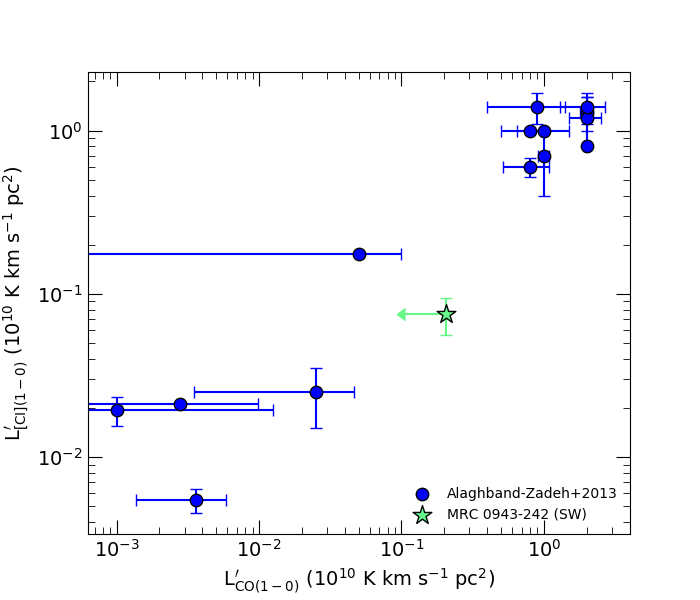
\includegraphics[width=0.8\columnwidth]{plots_chp4/CO_CI_HzRGs_AZ.png}
  \caption[$L'_{\rm [\ion{C}{i}](1-0)}$ vs $L'_{\rm CO(1-0)}$ of lensed dSFGs and HzRGs]{The magnification-corrected luminosities of [\ion{C}{i}](1-0), $L'_{\rm [\ion{C}{i}](1-0)},$ and CO(1-0), $L'_{\rm CO(1-0)},$ of lensed, dusty star-forming galaxies from \citet{Alaghband-Zadeh2013} are shown (circles). Additionally, the same luminosities are given for the off-nuclear [\ion{C}{i}](1-0) and CO(1-0) detection south-west of the host galaxy in MRC 0943-242 (star).}
  \label{fig:CO-CI-plot}
\end{figure}

\section{Discussion}
While no clear [\ion{C}{i}](1-0) line emission is detected at six out of seven of the host galaxies, one of the galaxies, TN J0121+1320, is detected. Additionally, several [\ion{C}{i}](1-0) detections are made at $d \sim 20 - 200$ kpc from the host galaxy nuclei - within their CGMs. The fact that we find more [\ion{C}{i}](1-0) detections in the halo should not be alarming. Several other studies have shown evidence for CO line emission at kpc-scale  distances from host galaxies well up to $d \sim 100$ kpc \citep[e.g.][]{Greve2004,deBreuck2005,Ivison2012,Emonts2014}. Such detections represent cold molecular gas that is primordial in origin and/or has yet to be accreted into the central regions of the galaxy haloes. 

Although the [\ion{C}{i}](1-0) flux detections that occur outside of the host galaxy are tentative, we are able to infer, from the [\ion{C}{i}](1-0) upper limits, the kinematics of the H$_2$ gas that they trace. Generally, the lines all have positive velocity shifts or are redshifted relative to the systemic velocity. The only exception being the line detection to the south-east of the host galaxy in 4C19.71 which is slightly blueshifted with a velocity shift of $\Delta \varv \simeq -4$ km s$^{-1}.$ The mean and median velocity offsets for all the off-nuclear detections are $\textlangle \Delta \varv \textrangle = 24$ km s$^{-1}$ and $\widetilde{\Delta \varv} = 16$ km s$^{-1}.$ The redshifts also all fall within $\Delta \varv \lesssim 70$ km s$^{-1}.$ Thus, the shift may be due to different ionisation conditions between the cold molecular ($T \simeq 10 - 20$ K) and warm, ionised gas regions ($T \simeq 10^4 - 10^6$ K). 

The [\ion{C}{i}](1-0) line-widths in the off-nuclear regions tend to fall well within the range of $\rm FWHM = 20 - 100$ km s$^{-1}.$ As we have already stated while discussing the individual sources, these observed line-widths clearly indicate that the gas is kinematically quiet. The only exception to this is the $z=3.52$ host galaxy of TN J0121+1320 which has a $\rm FWHM = 157 \pm 40$ km s$^{-1}$ indicative of gas possibly perturbed by turbulent motions associated with the AGN. 

The [\ion{C}{i}](1-0) line-widths of dusty SFGs and sub-milimetre (sub-mm) galaxies (SMGs) fall within the range of $\rm FWHM = 200 - 1000$ km s$^{-1}$ \citep{Alaghband-Zadeh2013,Bothwell2017}. Additionally, the line-widths of bright, lensed sub-mm galaxies in \citet{Nesvadba2019} are within the range of $\rm FWHM = 220 - 640$ km s$^{-1}.$ Hence, the cold molecular gas detected in the CGMs of the HzRGs in this sample are more relatively quiescent in comparison to the molecular gas detected in bright sub-mm galaxies at high-redshift.  

We also compare the H$_2$ masses of the host galaxies to those inferred from the off-nuclear [\ion{C}{i}](1-0) detections at $d\sim10-200$ kpc from the host galaxies. The mean and median of the H$_2$ masses for all of these detections are $\textlangle M_{\rm H_2} \textrangle = 5.53\e{9}$ M$_\odot$ and $\widetilde{M_{\rm H_2}} = 5.60\e{9}$ M$_\odot,$ respectively. Hence, off-nuclear H$_2$ mass measures are less than the upper limits in the host galaxies. This is possibly due to the off-nuclear or CGM H$_2$ being kinematically quiet relative to that of the host galaxy ISMs. 

The [\ion{C}{i}](1-0) non-detections at the host galaxies are consistent with HzRGs undergoing a period of quenching. In \citet{falkendal2019}, the host galaxies of radio-loud AGN at $z > 2$ are shown to be slightly below the Main Sequence of star-forming galaxies. In other words, their star-formation rates are unexpectedly low for their stellar-masses. The conclusion drawn from this observation is that a rapid consumption of molecular gas coupled with AGN-driven outflows are collectively responsible for the depletion of molecular gas in the HzRGs. The non-detection of H$_2$ tracers at the host galaxies also agrees well with the idea of HzRGs at $z > 2 - 3$ having already consumed most of their molecular gas by these redshift epochs. We also note that depletion time-scales for our sample of host galaxies are generally $\tau_{\rm depl} < 200$ Myr implying that a rapid consumption of molecular gas that occurred at earlier epochs may continue to deplete the gas rapidly, quenching the host galaxy's molecular gas supply. The H$_2$ gas reservoirs detected in the CGM may undergo infall into the host galaxy at a later epoch and refuel star-formation. 

The H$_2$ mass upper limits obtained for six of the seven HzRGs in the sample differ from those of the Spiderweb Galaxy (MRC 1138-262) \citep{emonts2018} and PKS0529-54 \citep{Man2019} which both have vast reservoirs of H$_2$ gas (inferred from [\ion{C}{i}]). Both galaxies have relatively high star-formation rates. The Spiderweb has a star-formation rate of $\rm SFR =1390 \pm 150$ M$_\odot$ yr$^{-1}$ while PKS 0529-54 also has a very vigorous star-formation rate of $\rm SFR = 1020^{+190}_{-170}$ M$_\odot$ yr$^{-1}.$ Gas-rich mergers may be responsible for the rapid star-formation as well as perturbed molecular gas kinematics traced by broad [\ion{C}{i}](1-0) lines in the Spiderweb Galaxy and PKS0529-54 host galaxies. No evidence of mergers are observed in the optical and infrared narrow and broad-band imaging of the HzRGs studied in this work, which may explain why they differ from the Spiderweb and PKS0529-54. 

\section{Conclusions}
%The last numbered section should briefly summarise what has been done, and describe
%the final conclusions which the authors draw from their work.

We have obtained ALMA bands 3 and 4 observations of seven radio galaxies with the aim of detecting neutral carbon, [\ion{C}{i}]$^3$P$_2 - ^3$P$_1$ ($\nu_{\rm rest} = 492.161$ GHz) which is a good tracer for molecular hydrogen (H$_2$). While no [\ion{C}{i}](1-0) line emission is detected in the interstellar mediums of six of the host galaxies, a [\ion{C}{i}](1-0) detection is made in the host galaxy TN J0121+1320 at $z=3.52.$ As a consequence, $3\sigma$ H$_2$ mass upper limits are obtained, assuming line-widths of 100 km s$^{-1}$ and are found to be approximately, M$_{\rm H_2}$/M$_\odot \lesssim 10^{10}.$ 

The ALMA data provides [\ion{C}{i}](1-0) line and continuum emission detections within the extended haloes of the galaxies at projected distances of $d\simeq 10 - 200$ kpc from the host galaxies, within the CGM. The H$_2$ gas reservoirs traced by these detections have on average $\textlangle M_{\rm H_2} \textrangle = 5.53\e{9}$ M$_\odot$ and line-widths between $\rm FWHM = 20 - 100$ km s$^{-1}.$ Comparing these line-widths to that of the host galaxy TN J0121+1320, $\rm FWHM = 157\pm40$ km s$^{-1},$ suggests that the molecular gas within the ISM of a galaxy is perturbed by rapid gas motions in the vicinity of the AGN. The molecular gas in the CGM, however, is kinematically quiet. Additionally, the ionised gas traced by \ion{He}{ii} is offset in velocity from [\ion{C}{I}](1-0) implying different ionisation conditions between the cold molecular and warm ionised gas.

The depletion time-scales for H$_2$ gas computed are well within the range of $\tau_{\rm depl} = 10 - 300$ Myr. If star-formation were to continue at the measured rate, then H$_2$ gas in the host galaxies would deplete very rapidly. This picture of the galaxies' eventual fate is consistent with the results of \citet{falkendal2019} who have shown that several high redshift radio galaxies (HzRGs) at $z>3$ appear to be in the process of quenching. 